\documentclass[12pt,letterpaper]{extarticle}
\usepackage[spanish,es-noshorthands]{babel}
\usepackage{lettrine}
\usepackage[table,dvipsnames]{xcolor}  % Combined xcolor options
\usepackage{hyperref}
\usepackage{booktabs}
% minted requires --shell-escape flag
% \usepackage{minted} % Commented out for now - requires pygmentize
\usepackage{siunitx}
\sisetup{detect-weight=true, detect-family=true, input-decimal-markers=., group-separator={,}, group-minimum-digits=4}

\AtBeginDocument{\RenewCommandCopy\qty\SI}

\usepackage{caption}

%%%%%%%%%%%%%%%%%%%%%%%%%%%%%%%%%%%%%%%%%%%%%%
%%%          Se incluye el preámbulo       %%%
%%%%%%%%%%%%%%%%%%%%%%%%%%%%%%%%%%%%%%%%%%%%%%
\usepackage{mathtools}
\usepackage{physics}
\usepackage[utf8]{inputenc}
% babel package is already loaded in main.tex, no need to duplicate
\usepackage{amsmath}
\usepackage{amssymb}
\usepackage{fancyhdr}
\setlength{\headheight}{14.5pt}
\decimalpoint
\usepackage{listings}
\usepackage{multicol}
\usepackage{tensor}
\usepackage{cancel}
\usepackage{sidecap}
\usepackage{setspace}
\usepackage{subcaption}
\usepackage{stix}
\usepackage{tikz}
% xcolor is already loaded in main.tex with options
\usepackage{pgfplots}
% cancel package already loaded above
\usepackage{geometry}
\usepackage{empheq}
\pgfplotsset{width=10cm,compat=1.9}
\usepackage[T1]{fontenc}
% hyperref already loaded in main.tex
\usepackage{titlesec, blindtext, color}
\definecolor{gray75}{gray}{0.75}
\newcommand{\hsp}{\hspace{20pt}}
\titleformat{\chapter}[hang]{\Huge\bfseries}{ \thechapter\hsp\textcolor{gray75}{|}\hsp}{0pt}{\Huge\bfseries}
\usepackage{tocloft}
\renewcommand{\cftsecleader}{\cftdotfill{\cftdotsep}}
\sidecaptionvpos{figure}{tl}

%%%%%%%%%%%%%%%%%%%%%%%%%%%%%%%%%%%%%%%%%
%%%%%      Underline Eqs        %%%%%%%%%
%%%%%%%%%%%%%%%%%%%%%%%%%%%%%%%%%%%%%%%%%

\newsavebox\MBox
\newcommand\Cline[2][red]{{\sbox\MBox{$#2$}%
  \rlap{\usebox\MBox}\color{#1}\rule[-1.2\dp\MBox]{\wd\MBox}{0.5pt}}}
%%%%%%%%%%%%%%%%%%%%%%%%%%%%%%%%%%%%%%%%%%
%%%        CONSTANTES                %%%%%
%%%%%%%%%%%%%%%%%%%%%%%%%%%%%%%%%%%%%%%%%%
\newcommand\mom{\sqrt{\frac{m\omega}{2\hbar}}}
\newcommand\momsq{\frac{m\omega}{2\hbar}}
\newcommand\dad{\s\begin{lstlisting}
import numpy as np

A = np.array([[1, 2],
              [3, 4]])
B = np.array([[0, 1],
              [2, 3]])
v = np.array([7, 9])        

AB = A @ B                  
R1 = AB + v                 
R2 = AB + np.broadcast_to(v, AB.shape)   

print("AB shape:", AB.shape, "\nAB:\n", AB)
print("v shape:", v.shape)
print("Resultado R1:\n", R1)
print("Resultado R2:\n", R2)

'''
En este código se ilustra cómo funciona el broadcasting en NumPy:

1. Se define una matriz A y otra B, y se calcula AB con producto matricial.
2. El vector v = (7,9) tiene forma (2,), que NumPy interpreta como (1,2). 
   Al sumarlo con AB (2,2), se expande automáticamente por filas: R1.
3. Con np.broadcast_to(v, AB.shape) se fuerza explícitamente una vista 
   de forma (2,2), que se suma a AB para dar R2.
4. Numéricamente R1 y R2 son iguales, pero internamente R2 utiliza 
   una vista broadcasted de solo lectura, compartiendo memoria con v.

En resumen, broadcasting permite que arreglos de distintas dimensiones 
se expandan virtualmente para realizar operaciones vectorizadas sin 
necesidad de copiar datos.
'''
\end{lstlisting}
qrt{\frac{m\omega\hbar}{2}}ie^{-\abs{z}^2/2}}
\newcommand\gus{\sqrt{\frac{\hbar}{2m\omega}}}
\newcommand\gussq{\frac{\hbar}{2m\omega}}
\newcommand\adag{\hat{a}^{\dagger}}
\newcommand\ah{\hat{a}}

\newcommand{\ylm}[2]{Y_{#1}^{#2}}
\newcommand{\fun}[3]{\Psi_{#1 #2 #3}(r,\theta,\phi)=R_{#1 #2}(r)Y_{#2}^{#3}(\theta,\phi)}
\newcommand{\funup}[3]{\Psi_{#1 #2 #3,\,+\frac{1}{2}}(r,\theta,\phi)=R_{#1 #2}(r)Y_{#2}^{#3}(\theta,\phi)}
\newcommand{\fundown}[3]{\Psi_{#1 #2 #3,\,-\frac{1}{2}}(r,\theta,\phi)=R_{#1 #2}(r)Y_{#2}^{#3}(\theta,\phi)}
%%%%%%%%%%%%%%%%%%%%%%%%%%%%%%%%%%%%%%%%%%%
%%%%     PALETA DE COLORES         %%%%%%%%
%%%%%%%%%%%%%%%%%%%%%%%%%%%%%%%%%%%%%%%%%%%
\definecolor{Verde}{HTML}{31B189}
\definecolor{Azul}{HTML}{7ACE67}
\definecolor{Naranja}{HTML}{FFC872}
\definecolor{Crema}{HTML}{FFE3B3}
\definecolor{AzulUV}{HTML}{1C36A1}
\definecolor{VerdeUV}{HTML}{00AA33}
\definecolor{RCimat}{HTML}{73243D}
\definecolor{GCimat}{HTML}{ACAAAB}




%%%%%%%%%%%%%%%%%%%%%%%%%%%%%%%%%%%%%%%%%%%%%%
%%%        Configuración bloques grises    %%%
%%%%%%%%%%%%%%%%%%%%%%%%%%%%%%%%%%%%%%%%%%%%%%
\usetikzlibrary{positioning, shapes}
\pgfdeclarelayer{background}
\pgfdeclarelayer{foreground}
\pgfsetlayers{background,main,foreground}
\usepackage{tcolorbox}
\tcbuselibrary{skins,breakable}
\usetikzlibrary{shadings,shadows}
\newenvironment{myblock}[1]{%
    \tcolorbox[beamer,%
    noparskip,breakable,
    colback=white,colframe=RCimat,%
    colbacklower=white!75!RCimat,%
    title=#1,
    coltitle = black]}%
    {\endtcolorbox}


    
\newtcbox{\othermathbox}[1][]{nobeforeafter, tcbox raise base, enhanced, sharp corners, colback=white!10, colframe=AzulUV!30!black,drop fuzzy shadow, left=1em, top=1em, right=1em, bottom=1em}

% Syntax: \colorboxed[<color model>]{<color specification>}{<math formula>}
\newcommand*{\colorboxed}{}
\def\colorboxed#1#{%
  \colorboxedAux{#1}%
}
\newcommand*{\colorboxedAux}[3]{%
  % #1: optional argument for color model
  % #2: color specification
  % #3: formula
  \begingroup
    \colorlet{cb@saved}{.}%
    \color#1{#2}%
    \boxed{%
      \color{cb@saved}%
      #3%
    }%
  \endgroup
}



%%%%%%%%%%%%%%%%%%%%%%%%%%%%%%%%%%%%%%%%%%%%%%
%%%          Para poner código en R        %%%
%%%%%%%%%%%%%%%%%%%%%%%%%%%%%%%%%%%%%%%%%%%%%%
\lstset{language=R,
    basicstyle=\fontsize{9}{10}\selectfont\ttfamily,
    stringstyle=\color{purple},
    otherkeywords={0,1,2,3,4,5,6,7,8,9},
    morekeywords={TRUE,FALSE},
    deletekeywords={data,frame,length,as,character},
    keywordstyle=\color{blue},
    commentstyle=\color{purple},
    showstringspaces=false
}


%%%%%%%%%%%%%%%%%%%%%%%%%%%%%%%%%%%%%%%%%%%%%%
%%%         Para código Python            %%%%
%%%%%%%%%%%%%%%%%%%%%%%%%%%%%%%%%%%%%%%%%%%%%%

\lstset{
  language=Python,
  basicstyle=\ttfamily\footnotesize,
  commentstyle=\color{red},
  keywordstyle=\color{blue},
  stringstyle=\color{orange},
  showstringspaces=false,
  breaklines=true,
  frame=single,
  columns=fullflexible
}

% --- Estilo personalizado para los outputs del modelo ---
\lstdefinestyle{mystyle}{
    language={},                     % No se usa ningún lenguaje
    backgroundcolor=\color{black!5}, % Un fondo gris muy claro
    basicstyle=\ttfamily\small,      % Fuente monoespaciada y pequeña
    breakatwhitespace=false,
    breaklines=true,                 % Rompe las líneas largas
    captionpos=b,                    % Posición del caption (abajo)
    keepspaces=true,
    showspaces=false,
    showstringspaces=false,
    showtabs=false,
    tabsize=2,
    frame=single,                    % Un marco sencillo alrededor
    framerule=0.5pt,
    rulecolor=\color{black!50},
    keywordstyle=\ttfamily,          % Palabras clave sin color especial
    stringstyle=\ttfamily,           % Strings sin color especial
    commentstyle=\ttfamily,          % Comentarios sin color especial
    literate={'}{{'}}1               % Trata ' como carácter normal
             {"}{{"}}1               % Trata " como carácter normal
}

% Note: cleveref must be loaded after amsmath (loaded in Preambulo)
\usepackage{cleveref}

%%%%%%%%%%%%%%%%%%%%%%%%%%%%%%%%%%%%%%%%%%%%%%
%%%          Datos de Encabezado           LaTeX Workshop is incompatible with  "vscode-pdf". We compete when opening a PDF file from the sidebar. Please consider disabling either extension.LaTeX Workshop is incompatible with  "vscode-pdf". We compete when opening a PDF file from the sidebar. Please consider disabling either extension.LaTeX Workshop is incompatible with  "vscode-pdf". We compete when opening a PDF file from the sidebar. Please consider disabling either extension.LaTeX Workshop is incompatible with  "vscode-pdf". We compete when opening a PDF file from the sidebar. Please consider disabling either extension.LaTeX Workshop is incompatible with  "vscode-pdf". We compete when opening a PDF file from the sidebar. Please consider disabling either extension.%%%
%%%%%%%%%%%%%%%%%%%%%%%%%%%%%%%%%%%%%%%%%%%%%%
\pagestyle{fancy}
\lhead{Tarea \#2}
\rhead{Procesamiento de Lenguaje Natural \& Visión Computacional}

%%%%%%%%%%%%%%%%%%%%%%%%%%%%%%%%%%%%%%%%%%%%%%
%%%      Configuración de los bloques      %%%
%%%%%%%%%%%%%%%%%%%%%%%%%%%%%%%%%%%%%%%%%%%%%%

% --- Numeración ---
\renewcommand{\thesection}{\arabic{section}}
\setcounter{secnumdepth}{1}   % Solo numera hasta \section
\setcounter{tocdepth}{3}      % Aún se listan en el TOC      

%%%%%%%%%%%%%%%%%%%%%%%%%%%%%%%%%%%%%%%%%%%%%%
%%%  Configuración de Tabla de Contenidos  %%%
%%%%%%%%%%%%%%%%%%%%%%%%%%%%%%%%%%%%%%%%%%%%%%
\rfoot{\hyperlink{MyToc}{\footnotesize{Tabla de contenidos}}}
\addto\captionsspanish{% Replace "english" with the language you use
  \renewcommand{\contentsname}%
    {Tabla de contenidos}%
}


\begin{document}


%%%%%%%%%%%%%%%%%%%%%%%%%%%%%%%%%%%%%%%%%%%%%%
%%%           Se incluye la portada        %%%
%%%%%%%%%%%%%%%%%%%%%%%%%%%%%%%%%%%%%%%%%%%%%%
\newgeometry{top=30mm, bottom=20mm, right=35mm, left=30mm}
% Cover page - packages already loaded in main document
% Additional tikz library for backgrounds
\usetikzlibrary{backgrounds}
% Declare the pgf layers
\pgfdeclarelayer{background}
\pgfdeclarelayer{foreground}
\pgfsetlayers{background,main,foreground}

% Definición de colores específicos para portada
\definecolor{rojoElectrico}{HTML}{FF4500}
% Note: RCimat and GCimat colors are redefined here with different values
% than in Preambulo.tex - consider using consistent colors
\definecolor{RCimatPortada}{HTML}{8B0000} 
\definecolor{GCimatPortada}{HTML}{FF4500}

\begin{titlepage}

% Fondo con TikZ
\tikz[remember picture,overlay] \node[opacity=1.0, inner sep=0pt] at ([yshift=-2.5cm]current page.south){
\begin{tikzpicture}
    \begin{pgfonlayer}{background}
        \filldraw[RCimatPortada] (-12,-8)--(-12,3)--(12,2)--(12,-8)--cycle;
    \end{pgfonlayer}

    \begin{pgfonlayer}{foreground}
        \filldraw[GCimatPortada] (-12,0)--(-12,1)--(12,1)--(12,0)--cycle;
    \end{pgfonlayer}
\end{tikzpicture}};

% Título
\par\noindent
{\bfseries\Huge Procesamiento de Lenguaje Natural \& Visión Computacional | Tarea \#2}
\vspace{0.2cm}

\par\noindent
\LARGE Generación y clasificación de texto con
arqutecturs de deep learning\\
\rule[0.3cm]{\linewidth}{2pt}

% Integrante
\vspace{0.5cm}
\begin{minipage}{0.6\textwidth}
    \begin{flushleft} \large
        {\emph{\textbf{César M. Aguirre Calzadilla}}}\\
    \end{flushleft}
\end{minipage}

% Logo y datos institucionales
\vspace{0.5cm}
\begin{center}
    
\includegraphics[scale=0.35]{Images/wordcloud_TOP.png}\par
    \vspace{1cm}
    {\textit{\bfseries\huge Centro de Investigación en Matemáticas}\par}
    \vspace{0.5cm}
    {\large Maestría en Cómputo Estadístico\par}
    % {\large Ciencia de Datos\par} % opcional
    \vspace{1cm}
\end{center}

% Profesores y fecha
\begin{center} \large
    {\emph{\textbf{Catedráticos:}}}\\
    \large Dr. Miguel Álvarez Carmona\par
    \large Dr. Ángel Ramón Aranda Campos\par
    \vspace{0.3cm}
    \large \today
\end{center}

\end{titlepage}
\restoregeometry%
\clearpage

%%%%%%%%%%%%%%%%%%%%%%%%%%%%%%%%%%%%%%%%%%%%%%
%%%        Tabla de Contenidos             %%%
%%%%%%%%%%%%%%%%%%%%%%%%%%%%%%%%%%%%%%%%%%%%%%
\hypertarget{MyToc}{}
\tableofcontents
\addtocontents{toc}{~\hfill\textbf{Página}\par}

%%%%%%%%%%%%%%%%%%%%%
%% Problemas      %%%
%%%%%%%%%%%%%%%%%%%%%
%\section{Modelos de Lenguaje}
\phantomsection\addcontentsline{toc}{section}{Modelos de Lenguaje}
\section*{Modelos de Lenguaje}

Un Modelo de Lenguaje, o LM por sus siglas en inglés, es un sistema probabilístico que asigna
una probabilidad a una secuencia de palabras, o bien, predice la probabilidad de aparición
de la siguiente palabra dado un contexto previo. Formalmente, un modelo de lenguaje define
una distribución sobre secuencias $\omega_1, \omega_2, \ldots, \omega_n$, de la forma:

\[
    P(w_1, w_2, \ldots, w_n) = \prod_{i=1}^n P(w_i \mid w_1, w_2, \ldots, w_{i-1}),
\]

Donde cada término $P(\omega_i \mid \omega_{<i})$ representa la probabilidad condicional de
la palabra $\omega_i$ dado su historia previa $\omega_{<i}$.

Los modleos de lenguaje tienen una larga tradición en el procesmaiento de lenguaje natural. 
Los primeros enfoques se basaron en modelos de n-gramas, que utilizan la suposición de Markov, i.e.
la probabilidad de una palabra depndiente únicamente de las últimas $n-1$ palabras de contexto. Por
ejemplo, un modelo de bigramas:

\[
    P(\omega_i | \omega_{<i}) \approx P(\omega_i | \omega_{<i})
\]

Estos modelos, aunque eran sencillos y computacionalmente eficientes, presentaban limitaciones claras
al no poder capturar depndencias de largo alcance, además de sufrir de "esparsidad", es decir,
muchas secuencias posibles nunca aparecían en los datos de entrenamiento. Es así como el 
desarrollo de técnicas de suavizado como Laplace o Kneser-Ney permitieron mejorar el desempeño de
los LM, pero no se resolvió por completo en cuanto a escasez de datos.

Tras el auge del Deep Learning demostrado en la última década, los modelos de redes neuronales 
reemplazaron a los modelos de n-gramas, pues estos eran capaces de aprender representaciones
continuas y modelar depndencias mucho más largas de texto. Al poco tiempo, los Transformers
cambiaron el paradigma y permitieron ampliar dicha capacidad, aprovechando del mecanismo de
self-attention para capturar relaciones globales en la secuencia, y a entrenar a muy graned escala
llegnado a lo que ahora conocemos como Large Language Models o LLM, como lo son GPT, BERT, LLama y 
todo el abanico de sucesores. 

El propósito central de un LM es estimar la probabilidad de una secuencia de palabras, locual lo convierte 
en una herramienta súmamente útil para una enorme cantida de tareas. Sin embargo, dado que todo LM 
asigna distribuciones de probabilidad sobre textom su calidad se mide en qué tan bien predice 
secuencias reales del idioma. El criterio intrínseco más utilizado para esta tarea de evaluación es
la perplejidad. 

%\section{Perplejidad}
\phantomsection\addcontentsline{toc}{section}{Perplejidad}
\section*{Perplejidad}

La Perplejidad (PPL) es la métrica estándar para evaluar modelos de lenguaje, especialmente
en tareas de predicción de secuencias. De manera intuitiva, PPL mide qué tan sorprendido
está un modelo frente a un conjunto de validación, cuanto mejor predice las palabras
reales que aparecen en el texto, menor será su perplejidad. 

Formalmente, para un conjunto de prueba $W = \omega_1, \omega_2,..., \omega_N$, la perplejidad
se define como:

\[
    \text{PPL}(W) = \exp \Big(- \frac{1}{N} \sum_{i=1}^{N} \text{log} p(\omega_i | \omega_{<i})\Big)
\]

La expresión anterior equivale a:

\[
    \text{PPL}(W) = \exp \Big(H(p,q) \Big)
\]

Donde $p(\omega_i | \omega_{<i})$ es la probabilidad asignada por el modelo para la palabra
$\omega_i$, dado el contexto anterior. 

Esta definición puede interpretarse como la media geométrica inversa de las probabilidades 
de que el modleo asigna a las palabras correctas. En consecuencia:

\begin{itemize}
    \item Una PPL baja implica que el modelo asigna alta probabilidad a las palabras reales, por
    lo que hay una mejor capacidad de predicción.
    \item Una PPL alta implica que el modelo se sorprende con frecuencia, entonces predice
    mal el texto.
\end{itemize}

Así entonces, la perplejidad equivale al número promedio de opciones equiprobables entre las
que el modelo ``cree'' tener que elegir en cada paso. Por ejemplo, una PPL = 3 significa que
el modelo se comporta como si en promedio tuviera que escoger entre tres palabras posibles
en cada posición.

La perplejidad está directamente relacionada con la entropía cruzada de la distribución
real frente a la estimada por el modleo. Es decir, minimizar la perplejidad equivale a 
maximizar la probabilidad del conjunto de validación. Por esta razón, se utiliza ampliamente
para comparar modelos de lenguaje entrenados con distintos algoritmos o configuraciones. 

Es importante destacar que:

\begin{itemize}
    \item No siempre correlaciona perfectamente con la calidad extrínseca de tareas como traducción automática o generación de texto, donde aspectos de coherencia semántica y adecuación estilística son también relevantes.
    \item La comparación entre modelos requiere que se use el mismo vocabulario y corpus de prueba; de lo contrario, las cifras no son conmensurables.
    \item Modelos con perplejidad baja pueden generar texto gramatical pero poco creativo (alta repetición), mientras que temperaturas de muestreo altas pueden producir lo opuesto: diversidad pero con mayor perplejidad.
\end{itemize}

\subsection{PPL en modelos de Redes Neuronales}

En arquitecturas modernas como RNN, LSTM, GRU o Transformers, el cálculo de la perplejidad se
implementa de manera directa a partir de la función de \textit{cross-entropy}. dado
que durante el entrenamiento se minimiza la entropía cruzada entre las etiquetas reales y la
distribución del modelo, evaluar la perplejidad en el conjunto de validación es equivalente a
medir el valor exponencial de dicha pérdida. 


\newpage
%%%%%%%%%%%%%%%%%%%%%%%%%%%%%%%%%%%%%%%%%%%%%%%%%%%%%%%%%%%%%%%%
%%%%%%%%%%%%%%%%%%%%%%%%%%%%%%%%%%%%%%%%%%%%%%%%%%%%%%%%%%%%%%%%
%%%%%%%%%%%%%%%%%%%%%%%%%% Enunciado %%%%%%%%%%%%%%%%%%%%%%%%%%%

\begin{myblock}
\phantomsection\addcontentsline{toc}{section}{Parte A | Generación de texto}
\section*{Parte A | Generación de texto}

    Reune al menos 100 canciones de tu género de música favorito. Unifica todo en un 
    solo archivo de texto (canciones.txt), separando cada canción con un delimitador claro. 
    Por ejemplo: <|startsong|> y <|endsong|> en una línea. 

    Además, normaliza con codificación UTF-8, elimina ruido (cabeceras repetidas, metadatos, 
    anuncios) y documenta tus decisiones de preprocesamiento.

\end{myblock}

%%%%%%%%%%%%%%%%%%%%%%%%%%%%%%%%%%%%%%%%%%%%%%%%%%%%%%%%%%%%%%%%
%%%%%%%%%%%%%%%%%%%%%%%%%%%%%%%%%%%%%%%%%%%%%%%%%%%%%%%%%%%%%%%%

%%%%%%%%%%%%%%%%%%%%%%%%%%%%%%%%%%%%%%%%%%%%%%%%%%%%%%%%%%%%%%%%
%%%%%%%%%%%%%%%%%%%%%%%%%%%%%%%%%%%%%%%%%%%%%%%%%%%%%%%%%%%%%%%%

Para esta tarea se reunieron canciones de la banda 'Twenty One Pilots'. Entre su discografía
se encuentran más de 100 canciones, que en general combinan composiciones y estructuras
del Hip Hop, Rap Rock, electropop y Synth-pop. En general es una banda que combina distintos
géneros, ritmos y estructuras, pero pensé que mantener un corpus de una misma banda podría
ser interesante. 

Para no descargar de manera manual las canciones, utilizamos la API de Genius. Genius es una 
página web dedicada a la captura y exposición de letras de canciones, así como a la colaboración
con fanáticos de las bandas para interpretar y dar explicación a fragmentos de las canciones. La
API de esta página permite, de manera sencila, acceder a su base de datos para sustraer las
letras que te interesen. Puedes realizarlo por título de canción, o por álbum, así como por artista
artista. La descarga de los datos es relativamente sencilla utilizando Python. 

El proceso de descarga se automatizó mediante un script, utilizando la biblioteca \texttt{lyricsgenius},
la cual funciona como un cliente para la API de Genius. La implementación se dividió en varias
fases clave para asegurar una recolección de datos robusta y limpia. 

Primero, se configuró el acceso a la API con un token de autenticación. Para refinar la calidad
de los datos edsde el inicio, se establecieron parámetros específicos en el cliente de \texttt{lyricsgenius}:

\begin{itemize}
    \item Se excluyeron términos como "Remix" y "Live" para evitar versiones alternativas de 
    las canciones y enfocarse en las letras de estudio.
    \item Se activó la opción \texttt{remove\_section\_headers} para eliminar automáticamente las
    las etiquetas estructurales de las letras (ej. \texttt{[Chorus]}, \texttt{[Verse]}), loaded
    cual representa un primer paso de preprocesamiento. 
\end{itemize}

Además de canciones por álbum se añadieron a la lista de descargas canciones que son sencillos 
de la banda, como 'Heathens' y 'Level of Concern'. Toda la información recolectada, es decir, el título
de la canción, el álbum y la letra, se almacenó en una estructura ed datos utilizando Pandas. 

Como último paso de limpieza en esta sección, se eliminaron posibles entradas duplicadas revisando el título
de las canciones. El resultado fue un corpus consolidado por un archivo en CSV llamado: \texttt{TOP\_lyrics\_hybrid.csv}.

\subsection{Limpieza para corpus generativo y para corpus clasificatorio}

Se tomó la decisión de realizar dos limpiezas de texto distinta: una para el caso de los modelos
generativos y otra para el caso de los modelos clasificatorios. Esto se realizó así por una
razón en particular, y es que en el caso generativo es importante mantener stop words y ciertas estructuras
musicales como los paréntesis para coros, dentro del corpus. Esto es así porque, idealmente, queremos
que nuestros modelos logren interpertar bien la estructura musical, ritmo y pacing tal cual
está estructurado en la letra sin modificaciones. 

Para el caso de los modelos clasificadores, se aplicará una limpieza más agresiva, quitando
stop words, pasndo todo a minúsculas y quitando arreglos que definan la estructura de canciones
como lo son 'chorus' 'verse' o 'bridege'. 

\subsection{Exploratorio del corpus}

Se realizó un exploratorio sencillo del corpus. Comenzamos por revisar qué palabras son las más frecuentes
en las canciones de Twenty One Pilots hasta el momento. 

\begin{table}[h!]
    \centering
    \caption{Las 15 palabras más frecuentes (sin *stopwords*).}
    \label{tab:frequent_words}
    \begin{tabular}{l c c}
        \toprule
        \textbf{Palabra} & \textbf{Frecuencia} & \textbf{Posición} \\
        \midrule
        don't & 627 & 1 \\
        know & 594 & 2 \\
        take & 300 & 3 \\
        time & 297 & 4 \\
        one & 288 & 5 \\
        like & 272 & 6 \\
        go & 241 & 7 \\
        tell & 227 & 8 \\
        need & 215 & 9 \\
        'cause & 205 & 10 \\
        save & 204 & 11 \\
        think & 193 & 12 \\
        say & 191 & 13 \\
        never & 189 & 14 \\
        'ive & 187 & 15 \\
        \bottomrule
    \end{tabular}
\end{table}

Destacan en el top 3 las palabras \textit{don't}, \textit{know}, \textit{take}, \textit{time}
y \textit{one}. Conociendo el contexto de la banda y el tipo de historias y narrativas que manejan
en sus canciones, estas cinco palabras tienen mucho sentido. Se trata de una banda que mantiene
una postura abierta respecto a los problemas de salud mental, la duda ante uno mimso, la incertidumbre
de la vida y la oscuridad que puede llegar a habitar nuestra mente. El discurso interno que mantiene
la banda nos reflea la duda, la ansiedad y la confusión. El término de \textit{time} puede ser 
una señal de preocupación ante el paso dle tiempo y cómo este infliuye en gran medida en los 
procesos personales y las luchas internas. 

Palabras como \textit{go}. \textit{tell}, \textit{need} y \textit{save} pueden apuntar a un sentido
de urgencia y la necesidad de acción. Son palabras de alta frecuencia, las cuales se alinean a la 
perfección con las letras que cuentan la lucha por seguir adelante o la necesdidad de ayuda. 

Creo que esto es un primer paso para el perfilado de autor en el ámbito de la lírica musical. Vemos
en estas palabras el estilo conversacional y confesional de las letras compuestas por Tyler Joseph. Las
canciones de Twenty One Pilots a menudo se sienten como un desgarro emocional y una confesión de
dolor, peligro o ayuda. Entonces, creo que hace mucho sentido esta lista. 

Podemos ver la gráfica de la ley de Zipf para las canciones de Twenty One Pilots en la figura
\ref{fig:Zipf_TOP}.

\begin{figure}[h!]
    \centering
    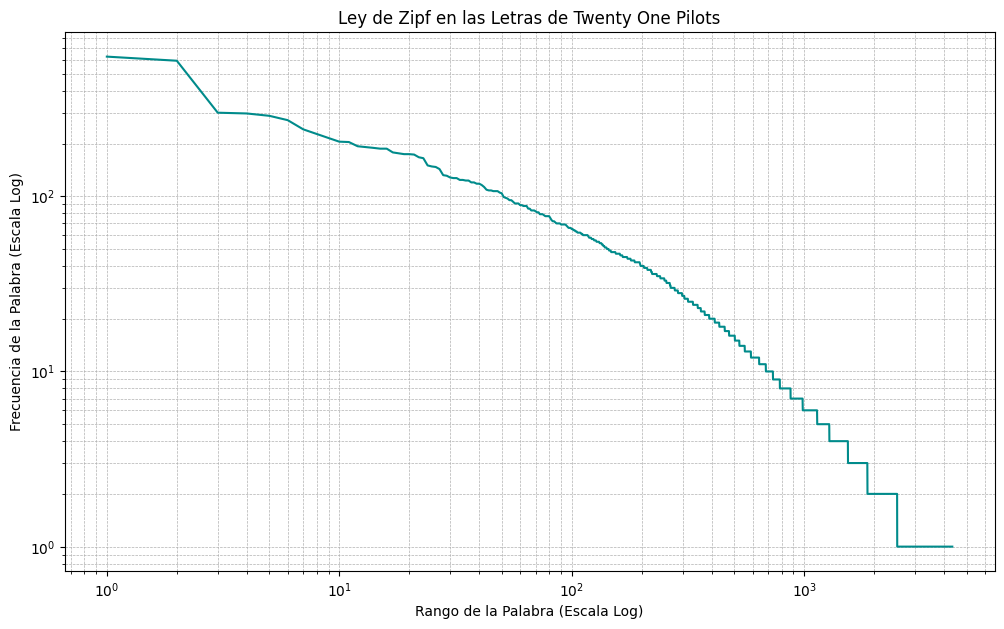
\includegraphics[width=0.8\linewidth]{Images/Zipf_TOP.png}
    \caption{Gráfica de la ley de Zipf para letras de Twenty One Pilots.}
    \label{fig:Zipf_TOP}
\end{figure}

De igual forma, podemos visualizar la frecuencia de las palabras de una manera más artística
implementando una wordcloud. 

\begin{figure}[h!]
    \centering
    
\includegraphics[width=0.8\linewidth]{Images/wordcloud_TOP.png}
    \caption{Wordcloud de Twenty One Pilots.}
    \label{fig:wordcloud_TOP}
\end{figure}

\clearpage






















\newpage
%%%%%%%%%%%%%%%%%%%%%%%%%%%%%%%%%%%%%%%%%%%%%%%%%%%%%%%%%%%%%%%%
%%%%%%%%%%%%%%%%%%%%%%%%%%%%%%%%%%%%%%%%%%%%%%%%%%%%%%%%%%%%%%%%
%%%%%%%%%%%%%%%%%%%%%%%%%% Enunciado %%%%%%%%%%%%%%%%%%%%%%%%%%%

\begin{myblock}
\phantomsection\addcontentsline{toc}{section}{Parte A | RNN}
\section*{Parte A | RNN}

    Entrena los modelos con las canciuones y con las arquitecturas RNN/LSTM/GRU. A nivel
    caracter y a nivel palabra.

\end{myblock}

%%%%%%%%%%%%%%%%%%%%%%%%%%%%%%%%%%%%%%%%%%%%%%%%%%%%%%%%%%%%%%%%
%%%%%%%%%%%%%%%%%%%%%%%%%%%%%%%%%%%%%%%%%%%%%%%%%%%%%%%%%%%%%%%%

%\begin{figure}[h!]
%   \centering
%   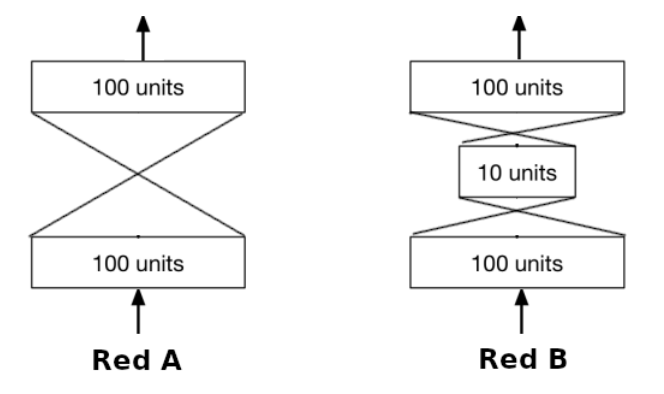
\includegraphics[width=0.8\linewidth]{Images/redA-redB.png}
%   \caption{Esquema de dos redes neuronales.}
%   \label{fig:redA_redB}
%\end{figure}


%%%%%%%%%%%%%%%%%%%%%%%%%%%%%%%%%%%%%%%%%%%%%%%%%%%%%%%%%%%%%%%%
%%%%%%%%%%%%%%%%%%%%%%%%%%%%%%%%%%%%%%%%%%%%%%%%%%%%%%%%%%%%%%%%

Los modelos de lenguaje (LM por sus siglas en inglés), buscan asignar probabilidades 
a secuecnias de palabras o caracteres y, en particular, estimar la probabilidad del 
siguiente token dado el contexto previo. Durante décadas, esto se abordó con n-gramas;
la métrica canónica es la perplejidad (PPL), la cual se definió como el exponencial de
la entropía cruzada priomedio, o de manera equivalente, es la inversa de la probabilidad
media del corpus. Minimizar la perplejidad es maximizar la probabilidad de los datos, y 
cuanto menor es la PPL, mejor el modelo en términos de sorpresa promedio por token. 

En ese sentido, las Redes Neuronales Recurrentes (RNN), introdujeron una forma distinta de trata el tiempo. Es decir, las RNN comparten pesos a lo largo de la secuencia y actualizan un estado oculto que "transporta" la información entre pasos, permitiendo modelar dependencias más largas que las que capturan n-gramas. Este paradigma dio paso a variantes con compuertas, que veremos más adelante, como lo son las LSTM y GRU. Fueron la piedra de inicio que también dio el primer paso para llegar a lo que ahora conocemos como Transformers y que son la base para los LLM. 

Aún así, las RNN y sus variantes siguen siendo fundamentales como baselines y por su valor didáctico, pues son la puerta de incio para el aprendizaje por secuencias y el Procesamiento de Lenguaje Natural con modelos de Redes Neuronales. 

\subsection{Formulación probabilística de los Modelos de Lenguaje (ML)}

Sea $\omega_1;T$ una secuencia. Un LM autoregresivo factoriza la probabilidad conjunta como:

\[
    p(\omega_{1;T}) = \prod_{t=1}^T p(\omega_t | \omega_{<t})
\]

Esta descomposición habilita el aprendizaje autosupervisado, i.e. donde cada paso temporal proporciona su propio "objetivo", de tal modo que $\omega_t$ se predice a partir de $\omega_{<t}$. El entrenamiento minimiza la entropía cruzada promedio (NLL), y la perplejidad se define como $\text{PPL} = \exp(\text{CE Promedio})$. 

Un procedimiento práctico asociado es el \textit{teacher forcing}: durante el entrenamiento, el modelo recibe como entrada el token veraddero del paso anterior y aprende a predecir el siguiente. 

\subsection{Arquitectura de las RNN}

En una RNN "simple", cada entrada $x_t$ (el embedding del token en $t$), actualiza el estado oculto $h_t$ con pesos compartidos.

En esta formulación, los parámetros de la red se organizan en tres matrices fundamentales que gobiernan el flujo de información:

\begin{itemize}
    \item $W_{xh}$ (a menudo denotada $U$) transforma la representación de entrada $x_t$ hacia el espacio del estado oculto.
    \item $W_{hh}$ (denotada en algunos textos como $W$) es la matriz recurrente que proyecta el estado oculto previo $h_{t-1}$ y permite transportar la información a lo largo de la secuencia.
    \item $W_{ho}$ (o $V$) mapea el estado oculto actual $h_t$ hacia el espacio de salida, produciendo los logits sobre el vocabulario.  
\end{itemize}

Estas matrices son compartidas en todos los pasos temporales, lo cual constituye la esencia de la recurrencia: el modelo reutiliza los mismos parámetros para procesar cualquier posición de la secuencia, logrando generalizar más allá de la ventana fija de los modelos n-grama.

\[
h_t = \phi(W_{xh}x_t + W_{hh} h_{t-1} + b_h) \;\;\;\;\;\;\;\;\;\; o_t = W_{h0}h_t + b_{o} \;\;\;\;\;\;\;\;\;\; \hat{y}_t = \text{Softmax}(o_t)
\]

Aquí, $\hat{y}_t$ es la distribución sobre sobre el vocabulario para le próximo token. Esta arquitectura se desenrolla en el tiempo para visualizar el flujo de información y de gradientes a lo largo de las secuencias. 

Acorde con Dan Jurafsky en el libro 'Speech and Language Processing', las  capas ocultas de los pasos anteriores funcionan a manera de memoria, o de contexto. Se trata de una especie de sistema que procesa la información para posteriormente tomar la decisión más adelante en el entrenamiento. Además, los pesos y el flujo tras cada capa lleva arrastrando todo el contexto anterior, no hay un límite en cuanto a la "cantidad" de contexto que se puede llevar cargando. Al menos en el modelo base de RNN. 

El entrenamiento de una RNN es un poco distinto al de un MLP tradicional. El backpropagation de las recurrentes sucede en dos pasos: primero se realiza inferencia hacia adelante, calculando tanto $h_t$ como $y_t$, y se acumula la pérdida tras cada avance a lo largo del tiempo, siempre guardando los valores de las capas ocultas tras cada paso para su uso posterior. Después, el segundo paso, es el procesamiento de la secuencia en reversa, donde se calculan lo sgradientes requeridois, logrando el cómputo y guardado dle término de error para usarlo en la capa oculta para cada paso hacia atrás. Jurafsky menciona que este proceso es llamado: "backpropagation a través del tiempo". 

Los modelos de lenguaje de las RNN procesan las secuencias de entrada una palabra a la vez. Es decir, lo que se intenta es predecir la palabra que sigue a partir de la palabra actual inmediata y el estado oculto anterior. Es por ello que las RNN se diferencían claramente de los n-gramas, pues estos tienen contexto limitado, y a diferencia del contexto fijo de modelos clásicos, son un sistema que no tiene límite de contexto en cuanto a todo lo que puede arrastrar desde sus secuencias de entrada iniciales. 


\subsection{Arquitectura Utilizada e Hiperparámetros}

Finalmente, para establecer una línea base de comparación, se implementó un modelo utilizando una Red Neuronal Recurrente simple (RNN). Aunque es susceptible al problema del desvanecimiento del gradiente en secuencias muy largas, su arquitectura más sencilla sirve como un punto de referencia fundamental para evaluar la ganancia en rendimiento obtenida con las arquitecturas más complejas de compuertas como GRU y LSTM.

Al igual que con los modelos anteriores, la configuración se mantuvo consistente para los entrenamientos a nivel de carácter y palabra.

\subsubsection{Estructura del Modelo}

La arquitectura del modelo RNN se diseñó con una mayor dimensionalidad en su estado oculto para compensar la simplicidad relativa de su unidad recurrente. La estructura fue la siguiente:

\begin{enumerate}
    \item \textbf{Capa de Embedding:} Una capa inicial para convertir los tokens de entrada en vectores densos. Se asumió una dimensión de embedding de 128 para mantener la consistencia con las otras arquitecturas.

    \item \textbf{Capas RNN Apiladas:} El núcleo del modelo consiste en 4 capas de RNN simple apiladas. Cada capa fue configurada con una dimensión de estado oculto (\texttt{hidden\_dim}) de 512 unidades, un tamaño mayor para aumentar la capacidad de representación del modelo.

    \item \textbf{Capa de Regularización (Dropout):} Se aplicó una tasa de \texttt{Dropout} del 30\% (0.3) entre las capas recurrentes para controlar el sobreajuste.

    \item \textbf{Capa de Salida (Clasificador):} Una capa lineal final proyecta la salida de la última capa RNN al tamaño del vocabulario, utilizando una función de activación \texttt{Softmax} para la predicción del siguiente token.
\end{enumerate}

\subsubsection{Hiperparámetros de Entrenamiento}

Los hiperparámetros utilizados para el entrenamiento del modelo RNN se detallan en la Tabla \ref{tab:rnn_hyperparams}. Se optó por un número menor de épocas de entrenamiento en comparación con los otros modelos, debido a la mayor rapidez con la que las RNN simples tienden a converger o a sobreajustar.

\begin{table}[h!]
    \centering
    \caption{Resumen de hiperparámetros de entrenamiento para el modelo RNN simple.}
    \label{tab:rnn_hyperparams}
    \begin{tabular}{l|l}
        \hline
        \textbf{Hiperparámetro} & \textbf{Valor Utilizado} \\ \hline
        Optimizador & \texttt{Adam} \\
        Tasa de Aprendizaje (Learning Rate) & \texttt{5e-4 (0.0005)} \\
        Función de Pérdida & \texttt{Cross-Entropy Loss} \\
        Tamaño del Lote (Batch Size) & \texttt{32} \\
        Épocas de Entrenamiento & \texttt{12} \\
        Semilla Aleatoria (Seed) & \texttt{42} \\ \hline
    \end{tabular}
\end{table}

\subsection{Resultados}

\begin{lstlisting}[
    style=mystyle,
    caption={Output crudo del modelo generativo a nivel de carácter.},
    label={lst:output-char-level}
]
I <UNK> <UNK> <UNK> <UNK> <UNK> <UNK> <UNK>  p l a n n e d  T h e r e ' s  s o m e o n e  e l s e ' s  d r e a m s ?  ( E l s e ' s  d r e a m s ?  ( E l s e ' s  d r e a m s ?  W h i n e  a l l ,  k n o w  T h a t  t h e y  t o l d  m e  I  w a s  g o n e  B u t  I ' l l  n e v e r  b e t t e r  o f f  m y  h e a d )  L e a r n i n g  d a r d y  s o  h a p p e n ?  W h a t  h a v e  a  c h a i n ' s  i c s  i n  y o u r  p a c e s ,  B l u r r y f a c e s  o f  f e e l i n '  s p u l l  s t i l l  a r e  s i t c i n g  G o t  t o  t h i s  t i m e  I ' l l  s i t  h e r e  ' t i l  I  f i n d  t h e  p r o b l e m  N o ,  I  m o v e  s l o w  I  w a n t  t o  s t o p  t i m e  I ' l l  s i t  h e r e  ' t i l  I  f i n d  t h e  p r o b l e m  N o ,  I
\end{lstlisting}

\clearpage

\begin{lstlisting}[
    style=mystyle,
    caption={Output crudo del modelo generativo a nivel de palabra.},
    label={lst:output-word-level}
]
<UNK> like my soul but not my mind is n't helping , saturday when it 's for the night 's decor it reveals what we dream of i have to know and i 'm a lot , right in one piece now i asked me , " son , when i grow old will you buy me a house of gold ? and when your father turns to stone will you take care of me ? " i will make you queen of everything you see i 'll put you on the map i 'm driving ' our thumbs for ammunition i was born a choker nobody 's comin ' for me comin ' for me from it 's decidin fine that part they form a lot with it 's real 'cause i told you you are out of my mind heard you say ( " today " 'cause the heat , place chances straight ever smell , you know that kills 's coming and welcome to the style you have n't seen in a while it 's lavish ( feeling gourmet ) welcome to the new way of living it 's just the beginning of lavish from the floor ( we 're broken too , yeah )
\end{lstlisting}

\subsubsection*{PPL por época}

\begin{figure}[h!] 
    \centering
    \caption{Comparación de la perplejidad (PPL) por época para los modelos RNN.}
    \label{fig:rnn_ppl_comparacion}

    \begin{subfigure}[b]{0.48\textwidth}
        \centering
        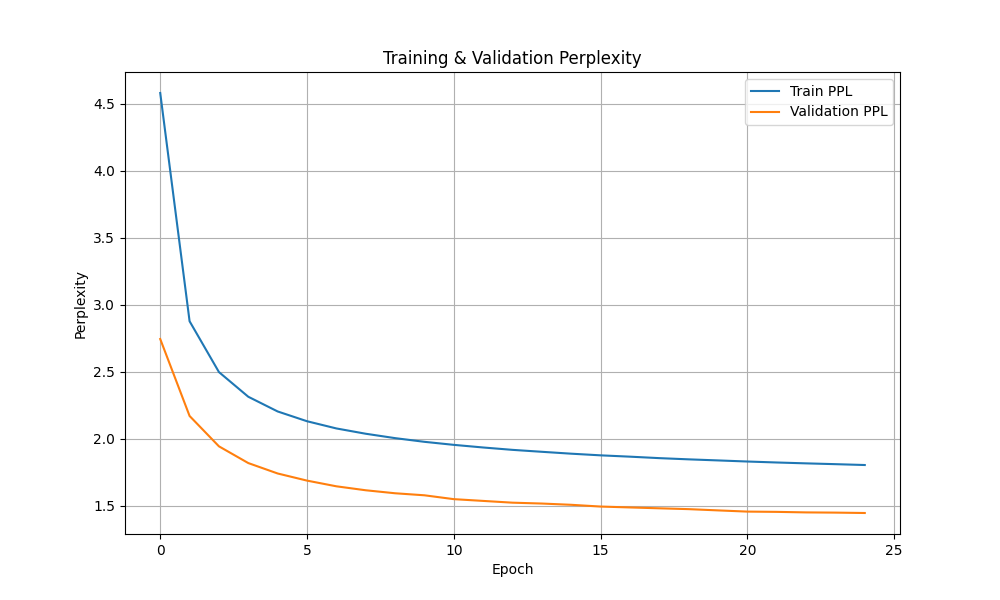
\includegraphics[width=\textwidth]{Images/rnn_training_history_c.png}
        \caption{Modelo a Nivel de Carácter.}
        \label{fig:rnn_ppl_char}
    \end{subfigure}
    \hfill % Este comando crea un espacio elástico entre las dos figuras
    \begin{subfigure}[b]{0.48\textwidth}
        \centering
        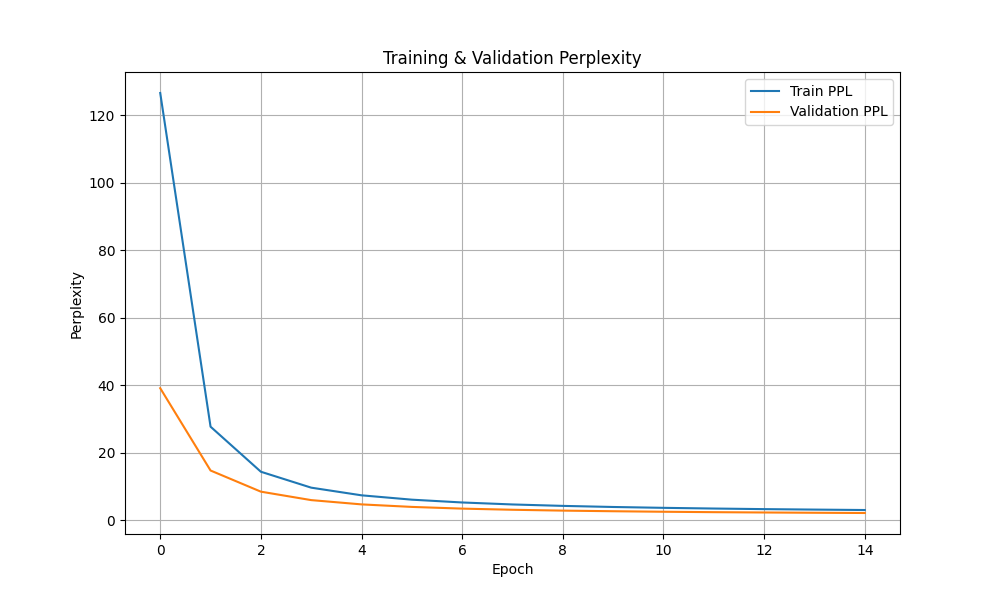
\includegraphics[width=\textwidth]{Images/rnn_training_history_w.png}
        \caption{Modelo a Nivel de Palabra.}
        \label{fig:rnn_ppl_word}
    \end{subfigure}
\end{figure}

\subsection{Conclusiones}

En primer lugar, podemos mencionar que los resultados de PPL muestran una clara diferencia
entre los modelos a nivel de carácter y a nivel de palabra. El modelo char-level alcanzó valores
de validación cercanos a 1.44 tras 25 épocas, indicando una buena capacidad de predicción local, 
aunque con salidas generativas afectadas por la presencia de múltiples \texttt{<UNK>}. Esto 
es muy probablemente debido a la forma en que se introdujo el promt inicial, pues no se tokenizó
a nivel carácter por carácter, lo que impidió al modleo explotar de manera correcta su estado
inicial. A pesar de ello, la disminución progresiva y estable de la PPL parece sugerir que el 
modelo aprendió bien acerca de regularidades ortográficas y patrones. 

Por otra parte, el modelo word-level presentó inicialmente una perplejidad muy alta, de hecho, 
superior a 100, pero convergió rápido hasta valores cercanos a 2.08 en el conjunto de validación.
Esto refleja que, aun con un corpus de tamaño limitado, las representaciones distribuidas de palabras
permiten capturar dependencias más semánticas y temáticas. Esta muestra refleja que a nivel palabras
hay una mejor coherencia y frases reconocibles dentro edl estilo lírico de Twenty One Pilots, 
aunque no sin redundancias y repeticiones frecuentes. 

La métrica de novelty confirma dichas tendencias. Los modelos LSTM y GRU (que veremos más adelante),
a nivel palabra, alcanzaron los valores más altos de novedad trigramal con $\sim 0.92$, mientras
que la RNN simple mostró mayor tendencia a memorizar, con un valor de 0.22 en trigramas. Esto implica
que las arquitecturas con puertas de memoria favorecen una mejor capacidad de recombinar fregmentos
de texto en lugar de limitarse a repetir secuencias vistas durante el enternamiento. 

En cuanto a la calidad cualitativa de las letras generadas, los outputs a nivel carácter tienden 
a generar secuencias ruidosas y poco interpretables, mientras que a nivel palabra están mejor
estructurados, con una mejor gramática, mejores referencias líricas y elementos estilísticos
asociado a la banda, aunque noto que esto provoca la repetición de frases que vuelve al modelo
poco creativo. Esto es reflejo de la limitaciones por el tamaño del corpus, provocando poca 
diveridad y la generacón de clichés.

Adelantandonos un poco a lo siguientes modelo, la RNN presentan mayor tendencia a memorizar 
y a repetir. Asimismo, la generación a nivel palabra logra capturar mejor el estilo y temática
del corpus. Ojalá tuvieramos mil canciones de Twenty One Pilots mas, para poder entrenar un LM
más solido. 



\clearpage











\newpage
%%%%%%%%%%%%%%%%%%%%%%%%%%%%%%%%%%%%%%%%%%%%%%%%%%%%%%%%%%%%%%%%
%%%%%%%%%%%%%%%%%%%%%%%%%%%%%%%%%%%%%%%%%%%%%%%%%%%%%%%%%%%%%%%%
%%%%%%%%%%%%%%%%%%%%%%%%%% Enunciado %%%%%%%%%%%%%%%%%%%%%%%%%%%

\begin{myblock}
\phantomsection\addcontentsline{toc}{section}{Parte A | LSTM}
\section*{Parte A | LSTM}

    Entrena los modelos con las canciuones y con las arquitecturas RNN/LSTM/GRU. A nivel
    caracter y a nivel palabra.

\end{myblock}

%%%%%%%%%%%%%%%%%%%%%%%%%%%%%%%%%%%%%%%%%%%%%%%%%%%%%%%%%%%%%%%%
%%%%%%%%%%%%%%%%%%%%%%%%%%%%%%%%%%%%%%%%%%%%%%%%%%%%%%%%%%%%%%%%

Uno de los principales problemas de las RNN es justo lo que volvió a aquella arquitectura una herramienta tan prometedora en los inicios del NLP como lo conocemos ahora: su contexto. Recordemos que las RNN arrastran el contexto de las capas de inicio, sin importar qué tan a profundidad vaya el entrenamiento. 

De acuerdo con Dan Jurafsky, entre las razones por las cuales las RNN no logran capturar, seleccionar y llevar adelante la información más importante es que se le solicita  alos pesos y a las capas ocultas que "proporcionen información útil para la decisión actual, y actualizar y llevar hacia adelante la información requerida para decisiones futuras". 

Además, justo ir cargando con toda la información previa, y realizar la retropropagación a lo largo del tiempo, sumando la pérdida de cada capa, paso a paso, provoca lo que se conoce como "desvanecimiento del gradiente". 

La solución a este tipo de problemas acarreados por las RNN llegó tras el diseño de arquitecturas que lograban no solo mantener contexto relevante a lo largo del tiempo, sino también lograr olvidar la información no necesaria, y recordar también la información requerida para el futuro. 

\begin{figure}[h!]
    \centering
    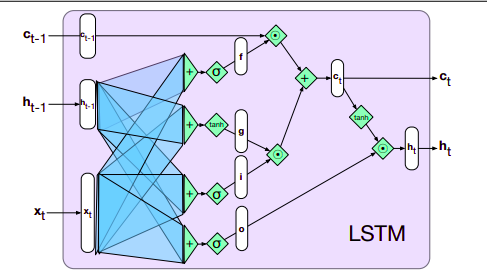
\includegraphics[width=0.8\linewidth]{Images/lstm-jurafsky.png}
    \caption{Arquitectura de una LSTM | Tomada de 'Speech Recognition' de Dan Jurafsky.}
    \label{fig:LSTM_arquitectura}
\end{figure}

Es así como se llegó a la creación de la Long Short-Term Memory (LSTM) o Red de Memoria a Largo y Corto Plazo. Este diseño no es nuevo, surgió en 1997, pero como muchas de las arquitecturas de Redes Neuronales, no fue sino hasta la década pasada que contamos con recursos suficientemente poderosos para poder entrenarlas y ponerlas en producción. 

Las LSTM realizan dos tareas principales: por un lado se encargan de eliminar información que ya no se necesita para el contexto, y por el otro lado capturan información que probablemente se utilice para la decisión siguiente. Este tipo de modelo logra aquello haciendo uso de una capa de contexto dentro de la arquitectura, además de las capas ocultas recurrentes propuestas en las RNN. Así, y mediante el uso de neuronas que utilizan compuertas para controlas el flujo de la información, logran hacer la captura del contexto relevante y no relevante. 

Dan Jurafsky lo explica de la siguiente manera: "las compuertas de una LSTM comparten un patrón de diseño común: cada una consiste en una capa de propagación hacia adelante, seguida de una función de activación sigmoide, seguida de una multiplicación elemento a elemento con la capa que se está controlando". Recordemos que la sigmoide es una función que "empuja" las salidas hacia el 0 o hacia el 1, de tal modo que al combinarla con multiplicaciones elemento a elemento, lo que estaremos logrando es poner en funcionamiento una máscara binaria que decide si los valores aprendidos en ese momento son eliminados o no. 

\subsection{Compuerta del Olvido (forget gate)}

Esta compuerta tiene como propósito eliminar información del contexto que ya es útil para la toma de decisiones futura. El proceso de eliminación es sencillo, se realiza una suma ponderada de la capa oculta del estado anterior y la entrada actual, para posteriormente pasarlo a una Sigmoide. Posteriormente, esta máscara binaria se multiplica elemento a elemento por el vector de contexto para eliminar la información que ya no es necesaria. Se define la multiplicación elemento a elemento como $\odot$, a este producto también le llamamos "producto de Hadamard". 

\[
   f_t = \sigma(U_f h_{t-1} + W_f x_t) 
\]

\[
    k_t = c_{t-1} \;\; \odot \;\; f_t 
\]

Ahora bien, para calcular la información que e va a extraer del estado oculto previo, y las 
entradas actuales, se utrilizac:

\[
  g_t = \text{tanh}(U_g h_{t-1} + W_gx_t)  
\]

\subsection{Compuerta de Adición (add gate)}

Para seleccionar la información que se agregará al contexto actual se utiliza la puerta de adición. Esta se define de la siguiente manera:

\[
    i_t = \sigma(U_i h_{t-1} + W_i x_t)
\]

\[
    j_t = g_t \;\; \odot \;\; i_t
\]

Y posteriormente sumamos esto al vector de contexto modificado para obtener nuestro nuevo vector de contexto:

\[
    c_t = j_t + k_t
\]

La compuerta de adición filtra la información nueva que está por ser añadida desde $g_t$. La diferencia clave entre la compuerta de adición y del olvido es sobre qué vector se aplican: la primera se aplica a la información nueva y la segunda se aplica al contexto previo. 

\subsection{Compuerta de Salida (output gate)}

La última compuerta en una LSTM base es la compuerta de salida. En ella se decide qué información se requiere para que el estado oculto actual. Es decir, este filtro lo que quiere hacer es tomar la decisión de que datos nos sirven para la decisión presente del modelo, no la que debe ser preservada para el futuro. Nuevamente, su estructura es similar a las anteriores:

\[
    o_t = \sigma(U_o h_{t-1} + W_o x_t)
\]

\[
    h_t = o_t \;\; \odot \;\; \text{tanh}(c_t)
\]


\subsection{Arquitectura Utilizada e Hiperparámetros}

De manera análoga al modelo GRU, se implementó y entrenó una arquitectura basada en redes de Memoria a Corto y Largo Plazo (LSTM, por sus siglas en inglés). La elección de LSTM permite una comparación directa con la arquitectura GRU, ya que ambas están diseñadas para mitigar el problema del desvanecimiento del gradiente en secuencias largas, aunque lo logran con mecanismos de compuertas (gates) ligeramente diferentes.

Nuevamente, la arquitectura se mantuvo idéntica para los entrenamientos a nivel de carácter y de palabra, con el fin de realizar una evaluación consistente.

\subsubsection{Estructura del Modelo}

El modelo LSTM se construyó con la siguiente configuración de capas:

\begin{enumerate}
    \item \textbf{Capa de Embedding:} Una capa inicial para mapear los tokens de entrada a vectores densos de 128 dimensiones.

    \item \textbf{Capas LSTM Apiladas:} El núcleo del modelo está compuesto por una pila de 6 capas LSTM, una configuración más profunda que la del modelo GRU para explorar la capacidad del modelo de aprender jerarquías de características más complejas. Cada capa cuenta con un estado oculto de 256 unidades.

    \item \textbf{Capa de Regularización (Dropout):} Se aplicó una tasa de \texttt{Dropout} del 30\% (0.3) entre las capas LSTM para prevenir el sobreajuste, una medida especialmente importante en arquitecturas más profundas.

    \item \textbf{Capa de Salida (Clasificador):} Una capa lineal final transforma la salida de la última capa LSTM al tamaño del vocabulario, empleando una activación \texttt{Softmax} para generar la distribución de probabilidad del siguiente token.
\end{enumerate}

\subsubsection{Hiperparámetros de Entrenamiento}

Los hiperparámetros de entrenamiento para el modelo LSTM se definieron como se muestra en la Tabla \ref{tab:lstm_hyperparams}. Notablemente, se utilizó un tamaño de lote mayor y un número superior de épocas en comparación con el modelo GRU para evaluar el comportamiento de la red bajo condiciones de entrenamiento más extensivas.

\begin{table}[h!]
    \centering
    \caption{Resumen de hiperparámetros de entrenamiento para el modelo LSTM.}
    \label{tab:lstm_hyperparams}
    \begin{tabular}{l|l}
        \hline
        \textbf{Hiperparámetro} & \textbf{Valor Utilizado} \\ \hline
        Optimizador & \texttt{Adam} \\
        Tasa de Aprendizaje (Learning Rate) & \texttt{5e-4 (0.0005)} \\
        Función de Pérdida & \texttt{Cross-Entropy Loss} \\
        Tamaño del Lote (Batch Size) & \texttt{64} \\
        Épocas de Entrenamiento & \texttt{15} \\ \hline
    \end{tabular}
\end{table}

\subsubsection*{PPL por época}

\begin{figure}[h!]
    \centering
    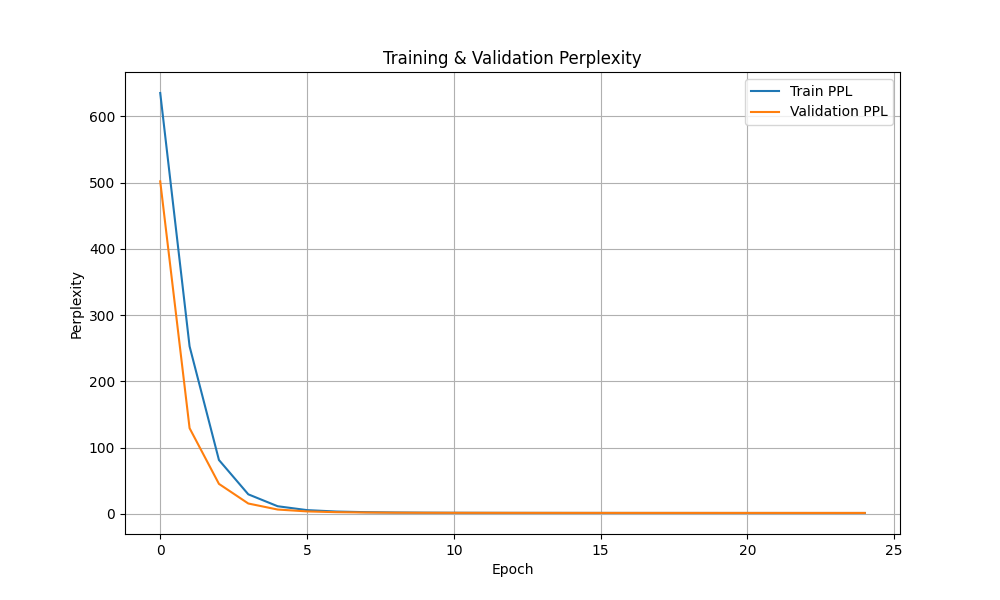
\includegraphics[width=0.7\textwidth]{Images/lstm_training_history_w.png}
    \caption{Modelo a Nivel de Palabra.}
    \label{fig:lstm_ppl_word}
\end{figure}

\subsection{Resultados}

\begin{lstlisting}[
    style=mystyle,
    caption={Output crudo del modelo LSTM a nivel de carácter.},
    label={lst:output-lstm-char}
]
I <UNK> <UNK> <UNK> <UNK> <UNK> <UNK> <UNK> s  w a y  t h a t  i t  s h o u l d  t o  l e t  t h i s  r e a t  I  d o n ' t  c a r e  w h a t ' s  i n  y o u r  h a i r  I  j u s t  w a n n a  k n o w  w h a t ' s  o n  y o u r  m i n d  I  u s e d  t o  s a y  I  w a n n a  d i e  b e f o r e  I ' m  o l d  B u t  b e c a u s e  o f  y o u ,  I  m i g h t  t h i n k  t w i c e  Y e a h ,  y e a h ,  y e a h !  Y e a h ,  y e a h ,  y e a h !  O h - o h - o h - o h - o h  Y e a h ,  y e a h ,  y e a h !  O h - o h - o h - o h - o h  Y e a h ,  y e a h ,  y e a h !  O h - o h - o h - o h - o h  Y e a h ,  y e a h ,  y e a h !  O h - o h - o h - o h - o h  Y e a h ,  y e a h ,  y e a h !  O h - o h - o h - o h - o h  Y e a h ,  y e a h ,  y e a h !  O h - o h - o h -
\end{lstlisting}

\begin{lstlisting}[
    style=mystyle,
    caption={Output crudo del modelo LSTM a nivel de palabra.},
    label={lst:output-lstm-word}
]
<UNK> like my soul but not my mind and you're living they recorded that up it) slowin' do i'm goin' all i feel some wonderin' would you be ( know you be? ) my soul 'cause is the only night, i know waging my side and the floor how my face some doors take i'm only yeah ( hates that she wrote he made in a binger and he live out if your passing gone it's another list and said my dream i'm pink, a car locomotive, and i didn't take it oh-oh-oh, they'r? asking for a second try you and i will never say it no, no, is not a little that's come up with start they're way same who-o-oa so us you've met but i am dying a friend, (ooh) home can won't you say that of a ride inspires you are not in a dream? neon waitin', wait, someone one oh, <EOS>
\end{lstlisting}

\subsection{Conclusiones}

El modelo LSTM, entrenado con un mayor número de épocas y un tamaño de lote superior al de 
GRU, mostró un desempeño robusto en términos de perplejidad. A nivel caracter, la PPL de validación
descendió de 7.75 en la primera época a valores cercanos a 1.15 en la época 12, mostrando una
notable capacidad de modelar dependencias locales en secuencias de símbolos. El output generado, 
aunque afectado por la presencia de tokens \texttt{<UNK>} de inicio, alcanzó una estructura
fonética y rítmica más clara, incluyendo patrones de repetición como ``\texttt{yeah, yeah, yeah}''. 
Si bien estos patrones son redundantes, reflejan rasgos estilísticos que no se presentaron en, por ejemplo,
el modelo de RNN. 

A nivel palabra, la PPL inicial fue muy alta, superior a los 600, pero decreció de maenra constante
hasta valores de validación cercanos a 2.24. Esto infica que el modelo aprendió a asignar probabilidades cada
vez más concentradas a secuencias posibles, aproximándose a un nivel de producción muy bueno. El texto
de output contiene frases de coherencia y con referencias reconocibles dentro del imaginario 
de la banda. Sin embargo, aún presenta estructuras fragmentadas y saltos semánticos abruptos. 

En cuanto a las métricas de novelty, el modelo LSTM alcanzó un equilibrio interesante. La 
proporción de novedad en trigramas fue de 0.92, muy cercana a la de la GRU, y superior la de la RNN.
Esto nos demuestra que, además de mantener memoria de secuencias frecuentes, la LSTM pudo recombianr
fragmentos de manera creativa, ecitando caer en mucha repetición. A nivel bigramas, se observó una tendencia
ligeramente mayor hacia la novedad con 0.65 puntos que confirman la capacida de explorar combinaciones nuevas sin
perder del todo la coherencia local. 

A nivel caracter, la PPL de este modelo es bastante bajo. A nivel palabra, la convergencia es lenta, pero
se sostiene al lograr niveles muy aceptables de PPl confirmando la utilidad del LSTM para
capturar tanto la semántica como la variedad léxica dentro de un corpus pequeño. Este modelo
supera a la RNN en cuanto a la reducción de la memorización y la maximización de la novelty. 
Sus resultados son comparables con los de la GRU, con ligera ventaja en coherencia global. 


















\clearpage





\newpage
%%%%%%%%%%%%%%%%%%%%%%%%%%%%%%%%%%%%%%%%%%%%%%%%%%%%%%%%%%%%%%%%
%%%%%%%%%%%%%%%%%%%%%%%%%%%%%%%%%%%%%%%%%%%%%%%%%%%%%%%%%%%%%%%%
%%%%%%%%%%%%%%%%%%%%%%%%%% Enunciado %%%%%%%%%%%%%%%%%%%%%%%%%%%

\begin{myblock}
\phantomsection\addcontentsline{toc}{section}{Parte A | GRU}
\section*{Parte A | GRU}

    Entrena los modelos con las canciuones y con las arquitecturas RNN/LSTM/GRU. A nivel
    caracter y a nivel palabra.

\end{myblock}

% \begin{figure}[h!]
%    \centering
%    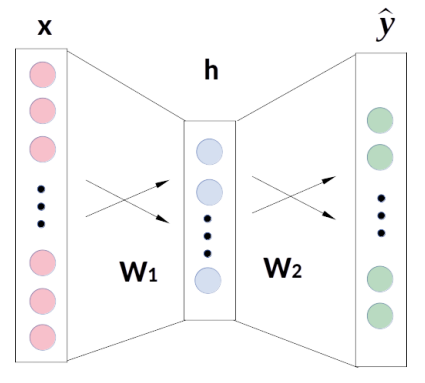
\includegraphics[width=0.4\linewidth]{Images/Red_Problema_02.png}
%    \caption{Red neuronal densamente conectada con una sola capa oculta.}
%    \label{fig:red_p02}
% \end{figure}

%%%%%%%%%%%%%%%%%%%%%%%%%%%%%%%%%%%%%%%%%%%%%%%%%%%%%%%%%%%%%%%%
%%%%%%%%%%%%%%%%%%%%%%%%%%%%%%%%%%%%%%%%%%%%%%%%%%%%%%%%%%%%%%%%

%%%%%%%%%%%%%%%%%%%%%%%%%%%%%%%%%%%%%%%%%%%%%%%%%%%%%%%%%%%%%%%%
%%%%%%%%%%%%%%%%%%%%%%%%%%%%%%%%%%%%%%%%%%%%%%%%%%%%%%%%%%%%%%%%

En el contexto de las RNN, sabemos que estas se mueven sin una ventana fija. El estado oculto $h_t$ resume el pasado y se actualiza con el nuevo $x_t$,. es decir, la palabra en la posición $t$, para predecir la salida $y_t$. En una RNN clásica, el cálculo se organiza en tres bloques: de la capa de entrada al estado oculto, del estado oculto a otro estado oculto, y de ese estado oculto a la salida. El entrenamiento del modleo de lenguaje s ehace por auto-supervisión con entropía cruzada como función objetivo, donde la probabilidad de la secuencia se factoriza paso a paso y se optimiza la pérdida. 

Sin embargo, RNN sufré del desvanecimiento del gradiente. Agregar compuertas como hace la LSTM resuelve ese problema al descartar información y decidir la que sí es de importancia para las decisiones. Dentro de la familia de RNN con compuertas se encuentra también la GRU. 

Conocida como Gated Recurrent Unit (GRU), este tipo de arquitecturas intenta mantener un desempeño competitivo con las LSTM a pesar de introducir menos parámetros. 

\subsection{La célula GRU y sus compuertas}

Una GRU controla el flujo de información con dos compuertas sigmoides por dimensión: la compuerta de actualización $z_t$ y  la compuerta de reinicio llamada $r_t$. La idea clave frente a la LSTM es que una sola compuerta gobierna a la vez el "olvido" del pasado y la decisión de escribir el nuevo estado, simplificando la arquitectura. 

Las ecuaciones de actualización son:

\begin{itemize}
    \item \textbf{Compuerta de actualización}: $z_t = \sigma(b_z + U_z x_t + W_z h_{t-1})$
    \item \textbf{Compuerta de reinicio}: $r_t = \sigma(b_r + U_r x_t + W_r h_{t-1})$
    \item \textbf{Candidato de estado}: $\hat{h}_t = \text{tanh}\Big(b + Ux_t + W(r_t \;\; \odot \;\; h_{t-1})\Big)$
    \item \textbf{Mezcla final}: $h_t = z_t \;\; \odot \;\; h_{t-1} + (1 - z_t) \;\; \odot \;\; \hat{h}_t$ 
\end{itemize}

La intuición detrás de esto es que $z_t$ implementa un integrador con fuga condicional. i.e. cerca de 1 "copia" el estado oculto $h_{t-1}$; mientras que cerca de 0 "reescribe" con $\hat{h}_t$. Por otra parte, $r_t$ decide cuánto del pasado participa en el cómputo del candidato $\hat{h}_t$, introduciendo no linealidad adicional a la relación entre lo pasado y lo futuro. 

A nivel estructural, la GRU mantiene los tres bloques U, W, V de una RNN, pero sustituye la transición oculta a oculta por una transición puerta a dependiente. Al compararse con una LSTM, la GRU elimina el estado de celda explícito y la salida está directamente en $h_t$. De esa manera, intenta ahorrar recursos volviendo a la GRU una LSTM "destilada". Ambos modelos suelen ser competitivos entre ellos, y su uso depende del problema específico a atender. 

\subsection{Arquitectura Utilizada e Hiperparámetros}

Para la tarea de generación de texto se implementó y evaluó un modelo basado en la arquitectura de Unidades Recurrentes Gated (GRU, por sus siglas en inglés). Esta arquitectura fue seleccionada por su eficiencia y su capacidad para capturar dependencias a largo plazo en secuencias, siendo una alternativa robusta a las redes LSTM.

El modelo fue entrenado tanto a nivel de carácter como a nivel de palabra para realizar una comparación exhaustiva. La arquitectura y los hiperparámetros se mantuvieron consistentes entre ambas modalidades para asegurar una evaluación justa de los resultados. A continuación, se detalla la configuración específica utilizada para los modelos GRU.

\subsubsection{Arquitectura del Modelo GRU}

El diseño del modelo se construyó como una pila de capas secuenciales, utilizando el framework \texttt{PyTorch}. La estructura fue la siguiente:

\begin{enumerate}
    \item \textbf{Capa de Embedding:} Una capa inicial que transforma los índices de los tokens (sean caracteres o palabras) en vectores densos. La dimensión de estos vectores de embedding se fijó en 128.

    \item \textbf{Capas GRU Apiladas:} El núcleo del modelo consiste en 4 capas GRU apiladas, cada una con una dimensión de estado oculto (\texttt{hidden\_dim}) de 256 unidades. El apilamiento de capas permite al modelo aprender representaciones de los datos a diferentes niveles de abstracción.

    \item \textbf{Capa de Regularización (Dropout):} Para mitigar el sobreajuste, se aplicó una capa de \texttt{Dropout} entre cada una de las capas GRU, con una tasa de desactivación de neuronas del 30\% (0.3).

    \item \textbf{Capa de Salida (Clasificador):} Finalmente, una capa lineal (densa) proyecta el estado oculto de la última capa GRU al tamaño del vocabulario, seguida de una función de activación \texttt{Softmax} para obtener una distribución de probabilidad sobre el siguiente token a predecir.
\end{enumerate}

\subsubsection{Hiperparámetros de Entrenamiento}

El proceso de entrenamiento fue configurado con los hiperparámetros que se resumen en la Tabla \ref{tab:gru_hyperparams}. La elección de estos valores se basó en una combinación de prácticas estándar y ajustes empíricos para la tarea.

\begin{table}[h!]
    \centering
    \caption{Resumen de hiperparámetros de entrenamiento para el modelo GRU.}
    \label{tab:gru_hyperparams}
    \begin{tabular}{l|l}
        \hline
        \textbf{Hiperparámetro} & \textbf{Valor Utilizado} \\ \hline
        Optimizador & \texttt{Adam} \\
        Tasa de Aprendizaje (Learning Rate) & \texttt{5e-4 (0.0005)} \\
        Función de Pérdida & \texttt{Cross-Entropy Loss} \\
        Tamaño del Lote (Batch Size) & \texttt{32} \\
        Épocas de Entrenamiento & \texttt{15} \\
        Semilla Aleatoria (Seed) & \texttt{42} \\ \hline
    \end{tabular}
\end{table}

\subsection{Resultados}

\begin{lstlisting}[
    style=mystyle,
    caption={Output crudo del modelo GRU a nivel de carácter.},
    label={lst:output-gru-char}
]
I <UNK> <UNK> <UNK> <UNK> <UNK> <UNK> <UNK>  v i s p e n s e  a n d  a b o v e  m y  t h r o a t ?  S h a d o w s  w i l l  s c r e a m  t h a t  I ' m  a l o n e - l o n e - l o n e  I - I - I - I ' v e  g o t  a  m i g r a i n e  A n d  m y  p a i n  w i l l  r a n g e  f r o m  u p ,  d o w n ,  a n d  s i d e w a y s  T h a n k  G o d  i t ' s  F r i d a y  ' c a u s e  F r i d a y s  w i l l  a l w a y s  b e  o n  a  s o n g  h e  w r o t e  T h i s  i s  t h e  l a s t  t i m e ,  t h i s  i s  t h e  l a s t  t i m e ,  t h i s  i s  t h e  l a s t  t i m e ,  t h i s  i s  t h e  l a s t  t i m e ,  t h i s  i s  t h e  l a s t  t i m e  E n t e r t a i n  m y  f a i t h  T h i s  i s  t h e  l a s t  t i m e ,  t h i s  i s  t h e  l a s t  t i m e
\end{lstlisting}

\begin{lstlisting}[
    style=mystyle,
    caption={Output crudo del modelo GRU a nivel de palabra.},
    label={lst:output-gru-word}
]
<UNK> like my soul but not my mind have i have back when a beautiful day but you me, around they will never don't want to know you who i see do i will you'll don't take a piece, of gold? to someone tryin' all next like what i wanna your footing, of nothing but i am i'll keep movin' a last feeling that come in black it's now what i know, up they get cold, sitting i get down) i get it's they just get to be all you never have it again never know they morph of a kingdom, join did a concert, i'll decorates with instead is a good progression catch i don't know i had to do one on my pride lean on my pride, i'm a lion i should the count i know the gesture we be slow i sing a day for break with a little cheetah after a re-beginning moment's mending memories dormant the beeps and tones keep would that not be 'cause me, are frozen and the mainland is climbing flying but we can the picture (am then my shirtsleeve shadows jacket not your wits then you mine to subliminally get out start (ooh-ooh) i don't go through you don't
\end{lstlisting}


\subsection{Conclusiones}

El modelo GRU mostró un comportamiento intermedio entre la simplicidad de la RNN y la capacidad
de memoria extendida de la LSTM. El comportamiento de la PPL demostró que, para este modelo 
de GRU, a nivel carácter descendió rápidamente hasta estabilizarse en valores bajos, los 
cuales fueron comparables con los alcanzados por la LSTM. En cuanto al texto generado, mostró
patrons fonéticos precisos y estructuras repetitivas con ritmo lírico, así como la toma de 
secuencias reconocibles de Twenty One Pilots como ``\textit{Shadows will scream that I'm alone}''
o ``\textit{I've got a migraine}'' de Holding On To You y de Migraine, ambas canciones muy populares 
de la banda. Esto demuestra que el modelo estaba un tanto limitado en cuanto a la creatividad,
pero que lograba encontrar secuencias líricas de importancia. 

Respecto a los resultados de la GRU a nivel palabra, la PPL mostró una disminución constante
hasta valoers relativamente bajos, aunque superiores a los alcanzados por la LSTM. Los outputs
generados reflejaron cierta coherencia temática, con construcciones gramticales mśa estbales que
las obtenidas por la RNN. Se observaron frases como ``\textit{i'll keep movin}''
o ``\textit{they morph of a kingdom}'', que si bien tenían una semántica clara, no se conectaban
del todo bien entre ellas. Esto refleja que nuestra GRU logra capturar contexto de medio alcance, 
que tiene dificultades con alcanzar la fluidez global de una LSTM. 

Los resultados de novelty confirman lo anterior. La GRU obtuvo una novedad en trigamas de 0.92,
la más alta en nuestros tres modelos de redes neuronales, pero en bigramas una de solo 0.62. Esto
nos parece estar diciendo que la arquitectura es especialmente efectiva para evitar repetición 
de manera excesiva, y explorar combinaciones nuevas sin sacrificar del todo la coherencia. Al 
compararlo con la RNN, se mostró una mayor memorización, mientras que el LSTM demuestra un balance
más equilibrado entre memoria novedad. 

De ese modo, podemos decir que la GRU es un modelo que cae justo en medio de la simpleza de la
RNN y sus problemas de memorización, y el entendimiento global y complejo de la LSTM. Es competivia
con la LSTM y supera claramente a la RNN. Quizás un modelo mejor regularizado, con un corpus 
más amplio y más tiempo de cómputo pueda demostrar ser una alternativa clara y eficaz a la LSTM.


%%%%%%%%%%%%%%%%%%%%%%%%%%%%%%%%%%%%%%%%%%%%%%%%%%%%%%%%%%%%%%%%
%%%%%%%%%%%%%%%%%%%%%%%%%%%%%%%%%%%%%%%%%%%%%%%%%%%%%%%%%%%%%%%

\clearpage
\phantomsection\addcontentsline{toc}{section}{Introducción a los Transformers y su relación 
con los LLM}
\section*{Introducción a los Transformers y su relación 
con los LLM}

Los modleos de lenguaje han recorrido un largo camino desde los enfoques estadísticos basados
en conteos de n-gramas hasta convertirse en los actuales modelos de lenguaje a gran escala, 
también conocidos como LLMs por sus siglas en inglés. En ese sentido, la arquitectura
Transformer (Vaswani et al., 2017) ha sido el principal punto de partida, con el cual se revolucionó la manera en
que presentamos y procesmaos secuencias linguísticas. 

A diferencia de los modelos recurrentes, como las RNN, LSTM o GRU, que procesan el texto paso 
a paso, y que sufrían de limitaciones para capturar dependencias largas, los Transformers 
incorporaron un mecanismo esencial para su éxito: la auto-atención (o \textit{Self-Attention}).
Este mecabnismo permite que cada palabra o token en una secuencia "se fije" de manera
directa en cualquier otro, sin importar la distancia que los separe, construyendo representaciones
contextuales mucho más ricas y globales. 

Este avance fue toda una revolución para el Procesamiento de Lenguaje Natural, pues creó 
modelos que podían manejar contextos extensos y aprender patrones complejos de manera eficiente. 
Como resultado, los Transformers se convirtieron muy rápidamente en la arquitectura dominante
en prácticamente todas las tareas del NLP, desde la traducción automática, hasta la generación 
de texto. 

Los LLMs contemporáneos como GPT, LLaMA, Gemini o DeepSeek no son más que instancias a gran
escala de esta arquitectura. Es decir, lo que se ha hecho es tomar la arquitectura y volverla
gigantesca, de tal modo que ahora tenemos modelos sumamente eficaces. La característrica de
\textit{Large} de los LLMs se refiere tanto a su número de parámetros como a la magnitud
del corpus con el que fue entrenado. Este diseño, que no necesita de convoluciones ni de 
recurrencia, representa un cambio de paradigma en la modelación del lenguaje. Se trata 
de una arquitectura altamente paralelizable y que puede capturar dependencias globales en el
texto de manera directa. 

\subsection{El cambio de paradigma}

El Transformer (Vaswani et al., 2017), es una arquitectura de red neuronal diseñada originalmente
para tareas de traducción automática, pero que pronto se convirtió en el estándar para el NLP, 
encontrando aplicaciones en muchos campos. 

A diferencia de los modelos recurrentes, que procesan de manera secuencial el texto, el Transformer
elimina la recurrencia y se basa en bloques paralelos compuestos de:

\begin{itemize}
    \item Mecanismo de self-atention o multi-head attention.
    \item Redes feed-forward posicionales.
    \item Normalización por capas y conexiones residuales.
\end{itemize}

En general, un Transformer puede adaptar tres variantes arquitectónicas principales:

\begin{itemize}
    \item \textbf{Decoder-only}: utilizado en modelos generativos como GPT, LLaMA o Mistral.
    \item \textbf{Encoder-only}: especializado en clasificación y comprensión como BERT, BETO o RoBERTa. 
    \item \textbf{Encoder-decoder}: comúnmente utilizados para traducción y tareas secuencia a secuencia.
\end{itemize}

Una de sus grandes ventajas es que pueden procesar contexto completo en paralelo, y aprender
dependencias de largo alcance en un solo paso, como no podrían los modelos recurrentes. 

\subsection{\textit{Self-Attention}}

Dado un conjunto de representaciones entrada $(x_1, x_2, \dots, x_n) \in \mathbb{R}^d$, una por 
cada token, la auto-atención produce nuevas representaciones $a_1, a_2, \dots, a_n$ donde cada
$a_i$ es una combinación ponderada de todos los vectores $x_j$ donde $j < n$.

La idea es que un token puede consultar información de otros tokens en función de su similitud
semántica y contextual.

Se definen tres proyecciones aprendidas de cada vector de entrada:

\[
    q_i = x_i W^Q, \;\;\;\;\;\;\; k_i = x_i W^K, \;\;\;\;\;\;\; v_i = x_i W^V
\]

Donde $W^Q, W^K, W^V \in \mathbb{R}^{d \times d_k}$ son matrices de parámetros.

La similaridad entre token $i$ (consulta) y otro token $j$ (clave) se calcula mediante un producto
punto escalado:

\[
    \text{score}(i,j) = \frac{q_i \cdot k_j}{\sqrt{d_k}}
\]

El uso del factor $\sqrt{d_k}$ estabiliza los gradientes y evita valores extremos al aplicar
la exponenciación en el softmax. Estas puntuaciones se normalizan con una Softmax, obteniendo
los pesos de atención:

\[
    \alpha_{ij} = \frac{\exp \Big(\text{score}(i,j)\Big)}{\sum_{m=1}^{n} \exp \Big(\text{score}(i,m)\Big)}
\]

Finalmente, la represebtación contextual del token $i$ se obtiene como una suma ponderada
de los valores:

\[
    \alpha_i = \sum_{j=1}^{n} \alpha_{ij} v_j
\]

Este mecanismo se aplica en paralelo para todos los tokens de la secuencia, generando la matriz
de salidas $A \in \mathbb{R}^{n \times d_v}$.

\subsection{\textit{Multi-head Attention}}

En la pr\'actica, no se utiliza una sola cabeza de atenci\'on, sino m\'ultiples. Con $h$ cabezas, se calculan diferentes subespacios de atenci\'on:

$$\text{head}_h = \text{Attention}(XW^Q_h, XW^K_h, XW^V_h)$$

y luego se concatenan todas las salidas para formar la representaci\'on final:

$$\text{MHA}(X) = [\text{head}_1; \dots; \text{head}_h] W^O$$

donde $W^O$ es una matriz de proyecci\'on adicional.

\subsection{Transformers populares}

La introducci\'on de la arquitectura Transformer no s\'olo transform\'o la investigaci\'on en PLN, sino que tambi\'en dio origen a una serie de modelos que hoy son considerados referentes en la evoluci\'on de los modelos de lenguaje a gran escala (\textbf{LLMs}). Entre ellos destacan las familias \textbf{GPT}, \textbf{LLaMA} y m\'as recientemente \textbf{DeepSeek}, cada una con enfoques y motivaciones distintas.

\subsubsection{GPT (Generative Pretrained Transformer)}

Los modelos GPT, desarrollados por OpenAI, constituyen el ejemplo paradigm\'atico de los Transformers decoder-only. Su entrenamiento se basa en la tarea de \textit{next-word prediction}, es decir, la predicci\'on autoregresiva de la siguiente palabra dada una secuencia de entrada.

\begin{itemize}
    \item \textbf{GPT-1 (2018)} introdujo la idea de preentrenar un gran modelo en corpus generales y luego ajustarlo (\textit{fine-tuning}) para tareas espec\'ificas.
    \item \textbf{GPT-2 (2019)} escal\'o el tama\~no (1.5B par\'ametros) y mostr\'o por primera vez capacidades generativas sorprendentes, aunque inicialmente fue liberado de forma parcial por preocupaciones de seguridad.
    \item \textbf{GPT-3 (2020)}, con 175B par\'ametros, consolid\'o el paradigma de los LLMs al mostrar \textit{emergent abilities}: razonamiento b\'asico, traducci\'on, generaci\'on de c\'odigo y di\'alogo. Su ajuste posterior dio origen a ChatGPT, que incorpor\'o \textit{instruction tuning} y \textit{reinforcement learning from human feedback} (RLHF) para mejorar su alineaci\'on con usuarios.
\end{itemize}

El impacto de GPT fue doble: estableci\'o la viabilidad de los LLMs en m\'ultiples dominios y mostr\'o que un \'unico modelo, entrenado con suficiente escala, puede generalizar a una amplia variedad de tareas ling\"u\'isticas sin redise\~nar la arquitectura.

\subsubsection{LLaMA (Large Language Model Meta AI)}

En 2023, Meta present\'o la familia LLaMA, concebida como un esfuerzo por abrir a la comunidad modelos competitivos pero con un enfoque en eficiencia y accesibilidad.

\begin{itemize}
    \item \textbf{LLaMA-1} ofrec\'ia variantes de 7B a 65B par\'ametros entrenadas con datos cuidadosamente filtrados.
    \item \textbf{LLaMA-2 (2023)} introdujo mejoras en el preentrenamiento y versiones afinadas para di\'alogo.
    \item \textbf{LLaMA-3 (2024)} alcanz\'o mayores tama\~nos (hasta 405B par\'ametros en versiones privadas), con una fuerte orientaci\'on a la investigaci\'on abierta y la compatibilidad con entornos de \textit{fine-tuning}.
\end{itemize}

Una de las principales contribuciones de la familia LLaMA fue democratizar el acceso a modelos de calidad comparable a GPT-3, pero bajo licencias abiertas, favoreciendo la investigaci\'on acad\'emica y el desarrollo de aplicaciones personalizadas.

\subsubsection{DeepSeek}

En el ecosistema m\'as reciente ha surgido DeepSeek, desarrollado en China como un competidor directo de modelos occidentales de gran escala. Su relevancia radica en dos aspectos:

\begin{itemize}
    \item \textbf{Optimizaci\'on computacional}: uso de t\'ecnicas avanzadas de entrenamiento distribuido que permiten reducir costos energ\'eticos y de hardware.
    \item \textbf{Competencia global}: representa un movimiento estrat\'egico en la carrera internacional de LLMs, mostrando que la arquitectura Transformer puede adaptarse a entornos con recursos limitados pero ambiciones de despliegue masivo.
\end{itemize}

DeepSeek no s\'olo apunta a competir en calidad, sino tambi\'en a abrir el camino a modelos m\'as eficientes, lo que sugiere que el futuro de los LLMs no depende \'unicamente de escalar par\'ametros, sino de optimizar su entrenamiento y uso.

\subsubsection{Otros modelos influyentes}

Aunque GPT, LLaMA y DeepSeek ocupan hoy el centro de atenci\'on, existen otras familias de Transformers fundamentales en la evoluci\'on del campo:

\begin{itemize}
    \item \textbf{BERT (2018)}: modelo \textit{encoder-only} basado en \textit{masked language modeling}, dise\~nado para tareas de comprensi\'on como clasificaci\'on, b\'usqueda sem\'antica y an\'alisis de sentimiento.
    \item \textbf{T5 (2019)}: modelo \textit{encoder-decoder} que formul\'o todas las tareas de PLN como problemas de traducci\'on de texto a texto.
    \item \textbf{Mistral (2023)}: modelos ligeros de arquitectura \textit{decoder-only}, altamente eficientes, dise\~nados para ser competitivos con menos par\'ametros.
    \item \textbf{Gemini (2023, Google DeepMind)}: sucesor de PaLM, con capacidades multimodales (texto e imagen) y mayor integraci\'on con entornos de b\'usqueda.
\end{itemize}
\newpage
%%%%%%%%%%%%%%%%%%%%%%%%%%%%%%%%%%%%%%%%%%%%%%%%%%%%%%%%%%%%%%%%
%%%%%%%%%%%%%%%%%%%%%%%%%%%%%%%%%%%%%%%%%%%%%%%%%%%%%%%%%%%%%%%%
%%%%%%%%%%%%%%%%%%%%%%%%%% Enunciado %%%%%%%%%%%%%%%%%%%%%%%%%%%

\begin{myblock}
\phantomsection\addcontentsline{toc}{section}{Parte A | TinyLLaMA-1.1B}
\section*{Parte A | TinyLLaMA-1.1B}

    Afinar al menos un modelo Transformer en cada parte (generación y clasificación), eligiéndolo
    de Hugging Face. 

\end{myblock}

%%%%%%%%%%%%%%%%%%%%%%%%%%%%%%%%%%%%%%%%%%%%%%%%%%%%%%%%%%%%%%%%
%%%%%%%%%%%%%%%%%%%%%%%%%%%%%%%%%%%%%%%%%%%%%%%%%%%%%%%%%%%%%%%%

%%%%%%%%%%%%%%%%%%%%%%%%%%%%%%%%%%%%%%%%%%%%%%%%%%%%%%%%%%%%%%%%
%%%%%%%%%%%%%%%%%%%%%%%%%%%%%%%%%%%%%%%%%%%%%%%%%%%%%%%%%%%%%%%%

%Los resultados de este problema se encuentran en los notebooks:

% \begin{itemize}
%     \item \textbf{MLP-MIR-Smooth.ipynb}
%     \item \textbf{exploratorio-mir-tarea01.ipynb}
% \end{itemize}

\subsection{Resultados}

\begin{lstlisting}[
    style=mystyle,
    caption={Output crudo del modelo TinyLLaMA-1.1B a nivel de palabra.},
    label={lst:output-gru-word}
]
I will take my heart with my hands and I'll lead you to believe that I am hiding something You don't need to run Heads are moving up and down, you got it It looks so much warmer there" <|startsong|> We used to play pretend, give each other different names I said I fly by the dangerous bend symbol (Wait, what? Wait, what?) And now they're outside, ready to bust (And guess what?) Lean on my pride, I'm a lion Pretending to understand how you think your world is ending (Keeps comin' around, keeps comin', keeps comin' ) I found my way, right time, wrong place But now you double as a paper maker <|endsong|> Mm, ba-da-dum, ba-da-dum-bum Dry us in the sand (Mm-mm) Da da, da da da, da-da) And when your father turns to stone <|endsong|> (Hey, hey, hey, hey, hey, hey, hey, hey) Just keep it outside, keep it outside, yeah Let me know when you've had enough Quarantine Ooh, ooh You should go your way, I should try mine Yeah\end{lstlisting}
\clearpage

\begin{lstlisting}[
    style=mystyle,
    caption={Output crudo del modelo TinyLLaMA-1.1B a nivel de palabra.},
    label={lst:output-gru-word}
]
If you ever wanna see me just let me know We get bodies every day (Ooh-ooh, ooh-ooh) Just don't believe the hype I don't have a chance to say goodbye I want to stop time Pardon my delay Don't make me waste my love Tell our dad I'm sorry I check the clock, wondering what he'll pull this time I've got two faces, Blurry's the one I'm not I've been thinkin' too much He knows that it's almost over <|endsong|> I know, I know-ow-ow And now they're outside, ready to bust (And guess what?) I could take the high road (Eh, eh, eh, eh) I prayed those lights would take me home They walked up to me and when they got close You'll be in and out, out, out, man They asked me, "Son, when I grow old Ooh, ooh So move out of our way, we're pushing sideways Yeah, yeah, yeah! Take that Know I'll keep movin', know I'll keep movin' Entertain my, entertain my faith But I know that I'm goin' low Low-key
\end{lstlisting}

\begin{lstlisting}[
    style=mystyle,
    caption={Output crudo del modelo TinyLLaMA-1.1B a nivel de palabra.},
    label={lst:output-gru-word}
]
Dema will fall like the other guys (I'll fake you out) I want to be afraid, but it seems that these days It's a backslide But they say a system's coming in In time, I will leave the city My friends and I have problems If I keep moving, they won't know You don't need to run But I can hear my way around Down there, it's some shelter from the weather They think this thing is a highway, highway I wanna see it all, no surprises, yeah Just so I don't fall through the floor So high, so high We used to play pretend, give each other different names Yeah, yeah, yeah! Don't forget abou-bou-bou-bou-bout me And now I just sit in silence To scrape the frosted windshield like we're barely scrapin' by Push on through Ah-ah-ah-ah-ah-ah, ah-ah-ah-ah-ah-ah, ah-ah-ah-ah-ah-ah (ah-ah-ah-ah-ah-ah) Can you save? Can you save my? Save my Are you doin' good? No, not me, it's for a friend (Ooh) Do-do-do
\end{lstlisting}

\subsection{Conclusiones}

El modelo TinyLLaMA-1.1B, a diferencia de las arquitecturas recurrentes tradicionales, mostró 
un desempeño significativamente superior en términos de perplejidad y calidad de los textos generados.
Tras un proceso de \textit{fine-tuning} ligero, con cuatro épocas y un \textit{batch size} de dos unidades,
la pérdida de entrenamiento descendió hasta valores cercanos a 0.61, lo cual corresponde
con una PPL de aproximadamente 1.84. En el conjunto de validación, la PPL se estabilizó 
en torno a un valor de 3.06, un valor muy bajo considerando la naturaleza del corpus. Estos resultados
superan claramente lo obtenido por las arquitecturas anteriores (RNN, LSTM y GRU), especialmente
a nivel de estabilidad y convergencia. 

En cuanto a la generación de letras, TinyLLaMA fue capaz de articular secuencias más largas y coherentes,
manteniendo tanto la estructura formal de las canciones como ciertos \textit{motifs} caracterísitcos
de Twenty One Pilots. Incrustó también conceptos que habitan el imaginario de la banda, como lo es
\textit{Blurryface}. A diferencia de las RNN, que tendieron a memorizar secuencias cortas, o las
GRU que mostraban fragmentación, TinyLLaMA logró mantener consistencia global incluso a lo largo
de estrofas enteras. 

Sin embargo, el moedlo también tiene limitaciones evidentes. Algunas secuencias derivaron en construcciones
fragmentadas o clichés genéricos como: ``\textit{I found my way, right time, wrong plac}'', una
sentencia importante y reconocida de la canción The Judge. Esto refleja que, a pesar de que 
el modelo aprovecha su capacidad de atención, sigue condicionado al tamaño relativamente pequeño
del corpus. La creatividad con la que se escribieron las canciones sigue siendo un tanto limitada, 
con muchas repeticiones que alteran la fluidez semántica por patrones rítmicos. 

En suma, podemos afirmar que TinyLLaMA-1.1B representa un salto claro en calidad frente a las arquitecturas
recurrentes. Su capacidad de auto-atención le permite modelar dependencias de largo alcance,
manteniendo tanto la coherencia semántica como los patrones rítmicos propios de las letras. Aunque
aún presenta clichés y algunas secuencias inconexas, la combinación de baja PPL, coherencia global y
estilo lírico consistente lo posicionan como un modelo superior. Quizás un corpus más extendo
y un ajuste más fino pueda superar ampliamente a esta implementación. 

Hablando en términos más coloquiales, es claro que incluso un Transformer básico y pequeño supera 
a las arquitecturas recurrentes, demostrando cómo es que este paradigma cambió la manera en que 
se hace el NLP de alto nivel. 

\clearpage
\newpage
%%%%%%%%%%%%%%%%%%%%%%%%%%%%%%%%%%%%%%%%%%%%%%%%%%%%%%%%%%%%%%%%
%%%%%%%%%%%%%%%%%%%%%%%%%%%%%%%%%%%%%%%%%%%%%%%%%%%%%%%%%%%%%%%%
%%%%%%%%%%%%%%%%%%%%%%%%%% Enunciado %%%%%%%%%%%%%%%%%%%%%%%%%%%

\begin{myblock}
\phantomsection\addcontentsline{toc}{section}{Parte A | Mistral-7B LoRA}
\section*{Parte A | Mistral-7B LoRA}

    Afinar al menos un modelo Transformer en cada parte (generación y clasificación), eligiéndolo
    de Hugging Face. 

\end{myblock}


%%%%%%%%%%%%%%%%%%%%%%%%%%%%%%%%%%%%%%%%%%%%%%%%%%%%%%%%%%%%%%%%
%%%%%%%%%%%%%%%%%%%%%%%%%%%%%%%%%%%%%%%%%%%%%%%%%%%%%%%%%%%%%%%%

\subsection{Mistral-7B LoRA}

Al ser este el modelo con mejores resultados, creí adecuado colocar un apartado más tecnico respecto
a este transformer. 

Mistral mantiene la arquitectura Transformer Decoder estándar, basada en \textit{Self-Attention}
y \textit{Feed-Forward Networks}, pero introduce modificaciones que reducen complejidad y aumentan
la eficiencia sin pérdida de capa expresiva. 

Recordemos que cada bloque de atención se define como:

\[
    \text{Attention}(Q,K,V) = \text{Softmax} \Big(\frac{QK^T}{\sqrt{d_k}+M}\Big) V
\]

Donde $M$ es la máscara causal que impide que el modelo ``mire a futuro''. Sin embargo, mistral 
modifica el mecanismo con dos adiciones:

\begin{itemize}
    \item \textbf{Sliding Window Attention (SWA)}: en lugar de atender a todos los tokens 
    previos, cada token solo atiende a los últimos $W$ tokens. Por defecto esto es $W = 4096$.
    Esto reduce la complejidad de $O(n^2)$ a $O(nW)$, permitiendo manejar contextos extensos
    con menor saturación de memoria. 
    \item \textbf{Grouped-Query Attention (GQA)}: esto reduce el número de cabezas de clave. En lugar
    de una proyección $(Q,K,V)$ por cabeza, agrupa varias cabezas de query y $h_{kv}$ las de 
    key; entonces $h_q < h_{kv}$. Esto reduce la memoria y el tiempo de inferencia sin sacrificar 
    la expresividad
\end{itemize}

Además, cada bloque Transformer incluye una red feed-forward con activación SiLU (Swish):

\[
    \text{FFN}(x) = W_2 \text{SiLU}(W_1x + b_1) + b_2
\]

Con dimension expansion factor de 4× el tamaño del embedding (similar a LLaMA). La función 
de activación SiLU (Sigmoid Linear Unit), conocdia también como Swish, es útil para Mistral poprque
combina lo mejor de ReLU con la Sigmoide, dando resultado a un entrenamineto más estable y un mejor 
rendimiento general del modelo. Esta se define matemáticamente como:

\[
    \text{SiLU}(x) = x \cdot \sigma(x) = x \cdot \frac{1}{1 + e^{-x}}
\]

A diferencia de ReLU, que tiene una esquina afilada con $x=0$, SiLU es una curva suave y continua. 
Esta suavidad le permite al proceso de optimización ser más estable durante el entrenamiento. De igual
forma se evitan cambios bruscos en los gradientes, permitiendo que el modelo converja de manera
más eficiente. Además, para valores negativos pequeños, la función decrece antes de volver a cero.

Asimismo, Mistral-7B LoRA cuenta con un entrenamiento previo sobre 7.3B de parámetros, y 32 
cabezas de atención. Como optimizador utiliza AdamW + cosine decay.  

Ahora bien, hablando de LoRA (Low-Rank Adaptation), este mecanismo permiote ajustar solo una 
pequeña parte de los parámetros del modelo sin modificar los pesos originales. La idea es que
se descomponga una actualización de $\delta W$ en cada matriz de pesos, transformandose en 
dos matrices de rango bajo:

\[
    W' = W + \delta W = W + BA \;\;\;\;\;\;\; A \in \mathbb{R}^{r \times d}, \; B \in \mathbb{R}^{d \times r}
\]

Donde el rango $r$ es pequeño, para nuestro caso específico fue $r = 16$, lo que implica entrenar
menos del 1\% de los parámetros totales. Esto reduce drásticamente el consumo de VRAM y permite ejecutar 
el fine-tuning completo en una sola GPU Titan RTX de 24 GB, que es lo que teníamos disponible
en el servidor de CIMAT Lab.

\clearpage

\subsection{Resultados}

\begin{lstlisting}[
    style=mystyle,
    caption={Output crudo del modelo Mistral-7B LoRA a nivel de palabra.},
    label={lst:output-mistral-word}
]
In the city lights I find myself
I don't know why
I wanna stay inside tonight
I think it's right
But my heart keeps telling me that I should go
Someplace I know where I belong
So, I take a deep breath, step outside
And follow my heart to where I want to hide

In the shadows of my memories
There's things I can't forget
The times when you and I used to be
Together we had what we wanted yet
A sparkle in our eyes would leave us
To chase dreams that only took us far from here
Now, all those years seem like a blur
And time has passed by, no trace left behind
Like footprints in the sand
My past steps slowly wash away
I see them sinking with the tide
Leaving me with a future I might not know

If you could read my mind
What would you think of who I am?
Have I changed since then?
Did your love bring out the best or the worst in me?
Do you remember how I felt?
\end{lstlisting}
\clearpage

\begin{lstlisting}[
    style=mystyle,
    caption={Output crudo del modelo Mistral-7B LoRA a nivel de palabra.},
    label={lst:output-mistral-word}
]
They say I'm broken but I'm breathing,
I say I'll heal but don't know what I mean
You see they say the heart never forgets,
The pain that you feel just gets passed down to me
And now it's like a game of catch,
Every time I move, the feeling gets passed along

Now we all talk about love and compassion,
But how can we show it when there's nothing left?
When every day feels more desperate than the last,
It's easy to believe what they say

They say, "Jena, there's something wrong with you,
Don't you get it yet? You're already gone,"
So I go looking for answers,
Looking for a cure, anything to be strong

"Jena, you're too broken, you won't get well,"
They say, "Your mind is lost and there's no way back"

Am I too far gone? Did I miss my chance?
Do you think maybe there's hope left?
\end{lstlisting}

\clearpage


\begin{lstlisting}[
    style=mystyle,
    caption={Output crudo del modelo Mistral-7B LoRA a nivel de palabra.},
    label={lst:output-mistral-word}
]
Sometimes my shadow sings louder than I do
A symphony of noise so loud it rings and echoes in the dark of night
It shines with light in its heart, and a deep soulful wisdom
The shadow was a creature of its own right
Sometimes we are just shadows of ourselves
Drowning in our own light as the real us watches on in the background
Someone else.
Some days I wake up and forget that I am me
And everything is a haze and then suddenly you're there
You bring back clarity

My best friend once told me that every person needs their best friend to see them for who they truly are
Every day I watch you and you help me to remember myself
When I look at your face I know the depths of your heart
Your eyes can tell stories and I love how you make me feel
I watch as you go about life, painting a masterpiece
One stroke at a time, coloring outside the lines, sometimes straying completely off course
But you never give up
And when I watch you, I feel like anything
\end{lstlisting}

\subsection{Conclusiones}

El modelo Mistral-7B LoRA mostró un gran desempeño y marcada mejora en la coherencia frente a las
arquitecturas tradicionales recurrentes y el resultado de TinyLLaMA. La pérdida promedio final 
fue de 1.59, lo que se traduce en una perplejidad de entrenamiento de 4.93, mientras que la PPL
de validación se estimó entorno a 5.7. Estras cifras reflejas una genración estable, con poco
sobreajuste, pese a realizarse solo en tres épocas, y el tamaño reducido del corpus. 

A nivel cualitativo, las letras generadas demustran una notable consistencia en cuanto a temática
y carga emocional. El texto del promt ``\textit{In the city lights I find myself}'' se muestra como una
canción con buena estructura lírica y estrofras, cerrando con un tono introspectivo ``\textit{Did your love bring out the best or the worst in me?
Do you remember how I felt?}''.  

La segunda canción,``\textit{They say I’m broken but I’m breathing}'' articula un discurso casi como 
de confesión, creo yo, imitando canciones como Cottonwood, Addict With A Pen o Fake You Out de 
Twenty One Pilots.  Finalmente,``\textit{Sometimes my shadow sings louder than I do}'' destaca por su
tono po´etico y met´aforas visuales, lo que sugiere que Mistral aprendi´o patrones 
estil´ısticos y tem´aticos complejos. Me parece que esto se ve impulsado por un buen promt, que
comparta el estilo y visión de la banda.

En comparación con TinyLLaMA-1.1B, Mistral produce versos más largos y mantiene una coherencia 
global más estable, aunque con una ligera pérdida de espontaneidad léxica. Creo que su ventana
de atención amplia y el uso eficiente de LoRA permitieron modelar dependencias de largo alcance
sin degradar la fluidez. 

Algo que pienso es que, aunque entrenamos con aproximadamente el 1\% de los parámetros con LoRa, el resto del
modelo, i.e. los 7 mil millones de parámetros de Mistral base, siguen determinando el comportamineto
de la distribución linguistica general de los outputs. Es decir, LoRA no borra el conocimiento previo
más bien lo modula a través de modificar un poco las matrices. Creo que por eso, sus salidas, aunque 
muy buenas e interesantes, no logran capturar por completo los clichés o estructuras más específicas
de Twenty One Pilots. Es decir, al final sigue siendo un LLM generalista, que ajusta los sesgos
de atención hacia patrones especídifcos. 

En consecuencia, Mistral se adapta y se combierte en un híbrido de estilo global por su entrenamiento
original y el estilo específico de mi corpus. Recordemos que por descomposición de LoRA: $W' = W + BA$.
Donde $B$ y $A$ son matrices de bajo rango (entrenables con menos del 1\% de los params.). Entonces, $W$
cofica todo el conocimiento general del modelo (con la gramática, semántica y razonamiento previo), y 
$BA$ es un filtro que ajusta a los tokens y define los patrones del modelo sobre los que se dará prioridad.

Se intenta reorientar lo aprendido. LoRA ``dobla'' el espacio de atencion, pero el punto de partida 
sigue siendo el embedding universal de Mistral. Esto, creo, explica por qué el modelo mantiene coherencia 
global y gramatical excelente, pero no siempre puede reproducir con fidelidad total el perfil 
artístico de Twenty One Pilots. Supongo que podríamos hacer más ajustes al finetuning para 
acercarnos cada vez más al estilo de Twenty One Pilots, pero eso se queda como trabajo futuro.


%%%%%%%%%%%%%%%%%%%%%%%%%%%%%%%%%%%%%%%%%%%%%%%%%%%%%%%%%%%%%%%%
%%%%%%%%%%%%%%%%%%%%%%%%%%%%%%%%%%%%%%%%%%%%%%%%%%%%%%%%%%%%%%%%

\clearpage
\newpage
%%%%%%%%%%%%%%%%%%%%%%%%%%%%%%%%%%%%%%%%%%%%%%%%%%%%%%%%%%%%%%%%
%%%%%%%%%%%%%%%%%%%%%%%%%%%%%%%%%%%%%%%%%%%%%%%%%%%%%%%%%%%%%%%%
%%%%%%%%%%%%%%%%%%%%%%%%%% Enunciado %%%%%%%%%%%%%%%%%%%%%%%%%%%

\begin{myblock}
\phantomsection\addcontentsline{toc}{section}{Parte B | CNN}
\section*{Parte B | CNN}

    Usando la misma base de la tarea 1, entrena un modelo por cada arquitectura: 
    CNN, RNN/LSTM/GRU, y un Transformer de Hugging Face con fine-tuning. Reporta
    accuracy y F1, incluye matriz de confusión y análisis de errores característicos.  

\end{myblock}

%%%%%%%%%%%%%%%%%%%%%%%%%%%%%%%%%%%%%%%%%%%%%%%%%%%%%%%%%%%%%%%%
%%%%%%%%%%%%%%%%%%%%%%%%%%%%%%%%%%%%%%%%%%%%%%%%%%%%%%%%%%%%%%%%

%%%%%%%%%%%%%%%%%%%%%%%%%%%%%%%%%%%%%%%%%%%%%%%%%%%%%%%%%%%%%%%%
%%%%%%%%%%%%%%%%%%%%%%%%%%%%%%%%%%%%%%%%%%%%%%%%%%%%%%%%%%%%%%%%

Las CNN para texto modelan \emph{n-gramas} como “filtros” que barren la secuencia de 
embeddings y extraen \emph{features} locales robustas (p. ej., negación corta, 
intensificadores). El \emph{max-over-time pooling} resume la activación más representativa 
por filtro, favoreciendo patrones discriminativos (\textit{salient n-grams}).

\subsection{Arquitectura CNN}

Sea $X \in \mathbb{R}^{L \times d}$ la matriz de embeddings (longitud $L$, dimensión $d$). Para un kernel 1-D de tamaño $k$:
\[
c_i = \sigma\!\big(\langle W,\, X_{i:i+k-1} \rangle + b\big), \quad
\mathbf{c} = [c_1,\dots,c_{L-k+1}], \quad
\hat{c} = \max(\mathbf{c})
\]
donde $W \in \mathbb{R}^{k \times d}$ y $\sigma$ es ReLU. Con varios tamaños de kernel $k \in \{2,3,4,5\}$ y $F$ filtros por tamaño, concatenamos 
$\hat{\mathbf{c}} = [\hat{c}^{(k_1)}, \ldots, \hat{c}^{(k_m)}]$ y proyectamos a $K$ clases:
\[
\hat{\mathbf{y}}=\mathrm{Softmax}\!\big(W_o \,[\hat{\mathbf{c}}] + b_o\big),\qquad
\mathcal{L} = \mathrm{CE}(\mathbf{y}, \hat{\mathbf{y}})
\]

Los kernels capturan patrones locales ($k{=}3$–$5$ suele alinear bien con bi/tri-gramas semánticos). El \emph{global max-pool} selecciona la evidencia más fuerte por filtro, 
haciéndolo robusto a la posición. Con reseñas 1–5, las frases muy positivas/negativas emergen como activaciones altas; las clases intermedias (2–3–4) requieren matices y suelen 
confundirse si la capacidad o el regularizador no están calibrados.

La arquitectura que realizamos fue TextCNN: embeddings 256, kernels $\{2,3,4,5\}$ o $\{3,4,5\}$, $F\in\{64,128\}$ filtros, \emph{dropout} (0.5–0.6), AdamW (LR $1\mathrm{e}{-3}$ o $2\mathrm{e}{-3}$), \emph{batch} 64, 20 épocas, 
\emph{early stopping} por F1-macro en validación. El \texttt{train\_cnn.py} guarda curvas de loss/F1, matriz de confusión y ROC OvR en el mejor punto, y usa 
class\_weights desde \texttt{meta.json}. :contentReference[oaicite:1]{index=1}

\subsection{Resultados}
\begin{table}[h!]
\centering
\caption{TextCNN — Resumen de experimentos en MeIA (polaridad 1–5).}
\label{tab:cnn_meia_transposed}
\begin{tabular}{lccc}
\toprule
\textbf{Parámetro} & \texttt{...\_f128\_do60} & \texttt{...\_f64\_k345\_do50} & \textbf{\texttt{...\_k345\_f128\_lr1e-3}} \\
\midrule
\textbf{Kernels}          & 2,3,4,5         & 3,4,5               & \textbf{3,4,5} \\
\textbf{Filtros}          & 128             & 64                  & \textbf{128} \\
\textbf{LR}               & $2\mathrm{e}{-3}$ & $2\mathrm{e}{-3}$   & \textbf{$1\mathrm{e}{-3}$} \\
\textbf{Dropout}          & 0.6             & 0.5                 & \textbf{0.5} \\
\textbf{Val F1-M}         & 0.414           & 0.425               & \textbf{0.456} \\
\textbf{Test Acc / F1-M}  & 0.374 / 0.357   & 0.410 / 0.379       & \textbf{0.448 / 0.441} \\
\bottomrule
\end{tabular}
\end{table}

\subsection{Visualización de Modelos}

% --- Figura 1: Matrices de Confusión ---
\begin{figure}[h!]
    \centering
    % Subfigura para el primer experimento
    \begin{subfigure}[b]{0.32\textwidth}
        \centering
        
\includegraphics[width=\textwidth]{/home/cesar/Natural-Language-Processing-and-Computer-Vision/Generacion-y-Clasificacion-de-Texto/Reporte/Images/CNN/exp_textcnn_f128_do60/confusion_test.png} % Reemplaza con la ruta de tu imagen
        \caption{\texttt{exp\_textcnn\_f128\_do60}}
        \label{fig:conf_exp1}
    \end{subfigure}
    \hfill % Para distribuir el espacio entre las subfiguras
    % Subfigura para el segundo experimento
    \begin{subfigure}[b]{0.32\textwidth}
        \centering
        
\includegraphics[width=\textwidth]{/home/cesar/Natural-Language-Processing-and-Computer-Vision/Generacion-y-Clasificacion-de-Texto/Reporte/Images/CNN/exp_textcnn_f64_k345_do50/confusion_test.png} % Reemplaza con la ruta de tu imagen
        \caption{\protect\texttt{exp\_textcnn\_f64\_k345\_do50}}
        \label{fig:conf_exp2}
    \end{subfigure}
    \hfill
    % Subfigura para el tercer experimento (el mejor)
    \begin{subfigure}[b]{0.32\textwidth}
        \centering
        
\includegraphics[width=\textwidth]{/home/cesar/Natural-Language-Processing-and-Computer-Vision/Generacion-y-Clasificacion-de-Texto/Reporte/Images/CNN/exp_textcnn_k345_f128_lr1e-3/confusion_test.png} % Reemplaza con la ruta de tu imagen
        \caption{\textbf{\texttt{exp\_textcnn\_k345\_f128\_lr1e-3}}}
        \label{fig:conf_exp3}
    \end{subfigure}
    \caption{Matrices de confusión para los tres experimentos de TextCNN en el dataset MeIA. Muestran la clasificación de polaridad (1-5).}
    \label{fig:confusion_matrices}
\end{figure}

\clearpage % Opcional: fuerza que la siguiente figura comience en una nueva página si el espacio es limitado

% --- Figura 2: Curvas ROC OVR ---
\begin{figure}[h!]
    \centering
    % Subfigura para el primer experimento
    \begin{subfigure}[b]{0.32\textwidth}
        \centering
        
\includegraphics[width=\textwidth]{/home/cesar/Natural-Language-Processing-and-Computer-Vision/Generacion-y-Clasificacion-de-Texto/Reporte/Images/CNN/exp_textcnn_f128_do60/roc_test.png} % Reemplaza con la ruta de tu imagen
        \caption{\texttt{exp\_textcnn\_f128\_do60}}
        \label{fig:roc_exp1}
    \end{subfigure}
    \hfill
    % Subfigura para el segundo experimento
    \begin{subfigure}[b]{0.32\textwidth}
        \centering
        
\includegraphics[width=\textwidth]{/home/cesar/Natural-Language-Processing-and-Computer-Vision/Generacion-y-Clasificacion-de-Texto/Reporte/Images/CNN/exp_textcnn_f64_k345_do50/roc_test.png} % Reemplaza con la ruta de tu imagen
        \caption{\protect\texttt{exp\_textcnn\_f64\_k345\_do50}}
        \label{fig:roc_exp2}
    \end{subfigure}
    \hfill
    % Subfigura para el tercer experimento (el mejor)
    \begin{subfigure}[b]{0.32\textwidth}
        \centering
        
\includegraphics[width=\textwidth]{/home/cesar/Natural-Language-Processing-and-Computer-Vision/Generacion-y-Clasificacion-de-Texto/Reporte/Images/CNN/exp_textcnn_k345_f128_lr1e-3/roc_test.png} % Reemplaza con la ruta de tu imagen
        \caption{\textbf{\texttt{exp\_textcnn\_k345\_f128\_lr1e-3}}}
        \label{fig:roc_exp3}
    \end{subfigure}
    \caption{Curvas ROC One-vs-Rest (OVR) para los tres experimentos de TextCNN. Se evalúa la capacidad de discriminación entre cada clase de polaridad y el resto.}
    \label{fig:roc_curves}
\end{figure}


\subsection{Conclusiones}

\begin{itemize}
    \item Centrar los kernels en tamaños de 3 a 5 mejora el rendimiento en comparación con usar un rango más amplio (2 a 5), ya que captura patrones semánticos más “limpios”.
    \item Reducir el Learning Rate a $1\mathrm{e}{-3}$ estabilizó el entrenamiento en el conjunto de validación y produjo el mejor modelo generalizado (F1-macro en test $=0.441$).
    \item Un valor de Dropout de 0.6 fue excesivo, ya que “acható” las distribuciones de probabilidad y degradó la métrica F1.
    \item Lamatriz de confusión muestra que los errores se concentran principalmente entre las clases adyacentes \emph{2–3–4} (la frontera ordinal), mientras que las clases extremas (1 y 5) mantienen un buen \emph{recall}.
    \item \emph{Nota:} Las gráficas de Confusión y ROC OvR se generaron automáticamente al guardar el mejor checkpoint del modelo.
\end{itemize}

El modelo basado en Convolutional Neural Networks (TextCNN) demostró un desempeño 
sólido como línea base para la clasificación de polaridad en reseñas turísticas. La mejor 
configuración —con kernels centrados en 3, 4 y 5 palabras, 128 filtros por tamaño, tasa de 
aprendizaje de $1\times10^{-3}$ y dropout de 0.5— alcanzó una precisión de 0.448 y un 
F1-macro de 0.441 en el conjunto de prueba, superando a las configuraciones previas con 
tasas de aprendizaje más altas o regularización excesiva. Se observó que el modelo captura
con efectividad las señales extremas de polaridad, es decir, las reseñas claramente 
positivas o negativas (clases 1 y 5), mientras que mantiene dificultades para distinguir
los matices intermedios (clases 2, 3 y 4), un fenómeno atribuible a la naturaleza ordinal
del problema y a la limitación inherente del pooling global en representar relaciones 
semánticas sutiles. Pese a ello, la TextCNN logra aprender representaciones 
discriminativas estables y generaliza adecuadamente al conjunto de validación, 
evidenciando que la optimización y la calibración del dropout son factores más 
determinantes que el aumento de filtros o la complejidad estructural. En síntesis, 
el modelo se consolida como un punto de partida robusto sobre el cual arquitecturas 
recurrentes o transformacionales podrán construir representaciones de contexto más
finas en etapas posteriores del análisis.

\clearpage
\newpage
%%%%%%%%%%%%%%%%%%%%%%%%%%%%%%%%%%%%%%%%%%%%%%%%%%%%%%%%%%%%%%%%
%%%%%%%%%%%%%%%%%%%%%%%%%%%%%%%%%%%%%%%%%%%%%%%%%%%%%%%%%%%%%%%%
%%%%%%%%%%%%%%%%%%%%%%%%%% Enunciado %%%%%%%%%%%%%%%%%%%%%%%%%%%

\begin{myblock}
\phantomsection\addcontentsline{toc}{section}{Parte B | RNN}
\section*{Parte B | RNN}

    Usando la misma base de la tarea 1, entrena un modelo por cada arquitectura: 
    CNN, RNN/LSTM/GRU, y un Transformer de Hugging Face con fine-tuning. Reporta
    accuracy y F1, incluye matriz de confusión y análisis de errores característicos.  

\end{myblock}

%%%%%%%%%%%%%%%%%%%%%%%%%%%%%%%%%%%%%%%%%%%%%%%%%%%%%%%%%%%%%%%%
%%%%%%%%%%%%%%%%%%%%%%%%%%%%%%%%%%%%%%%%%%%%%%%%%%%%%%%%%%%%%%%%

%%%%%%%%%%%%%%%%%%%%%%%%%%%%%%%%%%%%%%%%%%%%%%%%%%%%%%%%%%%%%%%%
%%%%%%%%%%%%%%%%%%%%%%%%%%%%%%%%%%%%%%%%%%%%%%%%%%%%%%%%%%%%%%%%

Recordemos que, a diferencia de las CNN, que capturan patrones locales posicionalmente invariantes, las RNN
procesan el texto de manera secuencial, manteniendo un estado oculto que teóricamente puede 
codificar información de todo el contexto previo. Para tareas de clasificación, este enfoque
permite modelar dependencias de largo alcance y el orden de las palabras. 

Una mejora realizada para las RNN base son las RNN Bidireccionales, que procesa la secuencia en ambas 
direcciones, tanto de izquierda a derecha, y de derecha a izquierda. Esto permite que el 
estado oculto en cualquier punto contenga información tanto del contexto pasado como del 
futuro, resultando en representaciones más ricas. 

\subsection{Arquitectura RNN}

Para obtener un único vector que representa toda la secuencia, se aplica una operación de pooling
sobre la secuencia de estados ocultos de la Bi-RNN. Si $H = [h_1, h_2,..., h_L]$ es la
secuencia de estados ocultos concatenados, donde cada $h_t$ combina el estado hacia adelante y 
hacia atrás, la representación final $h_{\text{pooled}}$ se obtiene como:

\[
    h_{\text{pooled}} = \text{Pool}(H)
\]

El vector resultante $h_{\text{pooled}}$ se pasa a una capa lineal final con una función de 
activación Softmax para la clasificación. La función de pérdida en este caso es la Entropía 
Cruzada, podnerada para manejar el desbalance de clases. Recordemos que en generación de texto, 
la métrica más usada de validación es la Perplejidad (PPL), que no es otra cosa más que la exponencial
de la Entropía Cruzada. 

\[
    \hat{y} = \text{Softmax}(W_o \cdot h_{\text{pooled}} + b_o) \;\;\;\;\;\;\;  L = \text{CrossEntropy}(y, \hat{y})
\]

Los modelos con los que experimentamos partieron de una base con capa de Bi-RNN y MaxPooling. al
oservar un sobreajuste significativo, con diferencia porcentuial de hasta 30 puntos de F1 entre 
training y validación, decidimos explorar diversas estrategias de regularización: aumento en 
el dropout, weight decay, label smoothing y diferentes estrategias de pooling como mean y maxpooling+mean, 
para intentar encontrar una mejor generalización.

\subsection{Resultados}

El primer modelo superó a la CNN, pero mostró un claro sobreajuste (Train F1 $\approx 0.78$ vs. Val F1 $\approx 0.47$). Los siguientes experimentos buscaron mejorar la regularización y explorar el impacto del mecanismo de \emph{pooling}.

\begin{table}[h!]
\centering
\caption{Bi-RNN — Resumen de experimentos en MeIA (polaridad 1–5).}
\label{tab:rnn_meia_transposed}
\begin{tabular}{lccc}
\toprule
\textbf{Parámetro} & \textbf{\texttt{...\_brnn\_five (baseline)}} & \texttt{...\_mean\_do60} & \texttt{...\_maxmean\_ls002} \\
\midrule
\textbf{Pooling}           & \textbf{max}          & mean                & max+mean \\
\textbf{Proj. Dropout}     & \textbf{0.5}          & 0.6                 & 0.5 \\
\textbf{Weight Decay}      & \textbf{$1\mathrm{e}{-4}$} & $2\mathrm{e}{-4}$   & $2\mathrm{e}{-4}$ \\
\textbf{Label Smoothing}   & \textbf{0.0}          & 0.05                & 0.02 \\
\textbf{Val F1-M}          & \textbf{0.467}        & 0.430               & 0.451 \\
\textbf{Test Acc / F1-M}   & \textbf{0.492 / 0.484} & 0.462 / 0.444       & 0.464 / 0.440 \\
\bottomrule
\end{tabular}
\end{table}

\subsection{Visualización de Modelos}

% --- Figura 1: Matrices de Confusión ---
\begin{figure}[h!]
    \centering
    % Subfigura para el primer experimento (el mejor)
    \begin{subfigure}[b]{0.32\textwidth}
        \centering
        % Reemplaza con la ruta de tu imagen
        
\includegraphics[width=\textwidth]{/home/cesar/project_b_t02nlp/models/rnn/exp_brnn_five/confusion_test.png} 
        \caption{\textbf{\texttt{exp\_brnn\_five}}}
        \label{fig:conf_rnn_exp1}
    \end{subfigure}
    \hfill 
    % Subfigura para el segundo experimento
    \begin{subfigure}[b]{0.32\textwidth}
        \centering
        % Reemplaza con la ruta de tu imagen
        
\includegraphics[width=\textwidth]{/home/cesar/project_b_t02nlp/models/rnn/exp_brnn_ls005_wd2e-4_mean_do60/confusion_test.png}
        \caption{\texttt{...\_mean\_do60}}
        \label{fig:conf_rnn_exp2}
    \end{subfigure}
    \hfill
    % Subfigura para el tercer experimento
    \begin{subfigure}[b]{0.32\textwidth}
        \centering
        % Reemplaza con la ruta de tu imagen
        
\includegraphics[width=\textwidth]{/home/cesar/project_b_t02nlp/models/rnn/exp_brnn_maxmean_ls002_wd2e-4_do50/confusion_test.png} 
        \caption{\texttt{...\_maxmean\_ls002}}
        \label{fig:conf_rnn_exp3}
    \end{subfigure}
    \caption{Matrices de confusión para los tres experimentos de Bi-RNN en el dataset MeIA. El modelo baseline (izquierda) muestra el mejor balance.}
    \label{fig:confusion_matrices_rnn}
\end{figure}

% --- Figura 2: Curvas ROC OVR ---
\begin{figure}[h!]
    \centering
    % Subfigura para el primer experimento (el mejor)
    \begin{subfigure}[b]{0.32\textwidth}
        \centering
        % Reemplaza con la ruta de tu imagen
        
\includegraphics[width=\textwidth]{/home/cesar/project_b_t02nlp/models/rnn/exp_brnn_five/roc_test.png}
        \caption{\textbf{\texttt{exp\_brnn\_five}}}
        \label{fig:roc_rnn_exp1}
    \end{subfigure}
    \hfill
    % Subfigura para el segundo experimento
    \begin{subfigure}[b]{0.32\textwidth}
        \centering
        % Reemplaza con la ruta de tu imagen
        
\includegraphics[width=\textwidth]{/home/cesar/project_b_t02nlp/models/rnn/exp_brnn_ls005_wd2e-4_mean_do60/roc_test.png}
        \caption{\texttt{...\_mean\_do60}}
        \label{fig:roc_rnn_exp2}
    \end{subfigure}
    \hfill
    % Subfigura para el tercer experimento
    \begin{subfigure}[b]{0.32\textwidth}
        \centering
        % Reemplaza con la ruta de tu imagen
        
\includegraphics[width=\textwidth]{/home/cesar/project_b_t02nlp/models/rnn/exp_brnn_maxmean_ls002_wd2e-4_do50/roc_test.png}
        \caption{\texttt{...\_maxmean\_ls002}}
        \label{fig:roc_rnn_exp3}
    \end{subfigure}
    \caption{Curvas ROC One-vs-Rest (OVR) para los experimentos de Bi-RNN. Evalúan la capacidad de discriminación de cada clase.}
    \label{fig:roc_curves_rnn}
\end{figure}


\subsection{Conclusiones}

\begin{itemize}
    \item La arquitectura Bi-RNN con MaxPooling superó al mejor modelo de mi TextCNN, estableciendo
    una nueva línea base con un F1-macro de 0.484.
    \item El mecanismo de pooling resultó ser el factor más determinante, MaxPooling fue superior
    a MeanPooling y a la concatenación \texttt{max+mean}. Esto nos está indicando que para este problema
    las señales con alta carga semántica son más informativas que la evidencia contextual distribuida por
    el texto. 
    \item Los intentos de regularización más agresiva, como label smoothing, o un mayor weight decay, 
    fueron contraproducentes. Suavizar las predicciones parece diluir las distinciones sutiles entre las
    clases intermedias (2-3-4), empeorando el rendimiento general. 
    \item Al igual que con la CNN, el desafío principal es la zona media de la polaridad, las clases
    intermedias ya mencionadas. Aunque el modelo captura bien los extremos (1 y 5), la naturaleza ordinal
    y la ambiguedad semántica de las puntuaciones intermedias son la principal causa de error.
\end{itemize}

Este modleo basado en una RNN bidireccional demostró ser más efectivo que la convolucional para capturar
el contexto secuencial de las reseñas. La mejor configuración, una Bi-RNN con MaxPooling sobre los 
estados ocultos y una regularización moderada obtuvieron los mejores resultados de las pruebas, con un
accuracy de 0.492, y un F1-Macro de 0.484 en el conjunto de prueba. El análisis de los experimentos
revelaron que la estrategia de Pooling fue la que más eficientemente abordó el problema, el uso de 
MaxPooling logra identificar características secuenciales más destacadas, lo cual fue benéfico para
promediar la evidencia a lo largo de toda la secuencia, que tendía a centralizar las prediciones. 

Pese a las mejoras, este modelo aún comparte el problema de la zona media, con las etiquetas de polaridad
(2-3-4). La Bi-RNN se establece como una línea base sólida, confirmando que el modelado del 
orden secuencial puede aportar información de valor, y siendo un excelente punto de partidad para evaluar
el portencial de arquitecturas basadas en atención como los Transformers. 








\clearpage
\newpage
%%%%%%%%%%%%%%%%%%%%%%%%%%%%%%%%%%%%%%%%%%%%%%%%%%%%%%%%%%%%%%%%
%%%%%%%%%%%%%%%%%%%%%%%%%%%%%%%%%%%%%%%%%%%%%%%%%%%%%%%%%%%%%%%%
%%%%%%%%%%%%%%%%%%%%%%%%%% Enunciado %%%%%%%%%%%%%%%%%%%%%%%%%%%

\begin{myblock}
\phantomsection\addcontentsline{toc}{section}{Parte B | LSTM}
\section*{Parte B | LSTM}

    Usando la misma base de la tarea 1, entrena un modelo por cada arquitectura: 
    CNN, RNN/LSTM/GRU, y un Transformer de Hugging Face con fine-tuning. Reporta
    accuracy y F1, incluye matriz de confusión y análisis de errores característicos.  

\end{myblock}

%%%%%%%%%%%%%%%%%%%%%%%%%%%%%%%%%%%%%%%%%%%%%%%%%%%%%%%%%%%%%%%%
%%%%%%%%%%%%%%%%%%%%%%%%%%%%%%%%%%%%%%%%%%%%%%%%%%%%%%%%%%%%%%%%

%%%%%%%%%%%%%%%%%%%%%%%%%%%%%%%%%%%%%%%%%%%%%%%%%%%%%%%%%%%%%%%%
%%%%%%%%%%%%%%%%%%%%%%%%%%%%%%%%%%%%%%%%%%%%%%%%%%%%%%%%%%%%%%%%

Si bien la arquitectrura interna de la celda LSTM es la misma tanto para 
generación de texto como para clasificación de texto, el objetivo final, y la
estructura del modelo, cambian. 


\subsection{Arquitectura LSTM}

En la tarea de generación, el modleo funciona como un Language Model. El objetivo
es predecir el siguiente token de la secuencia $y_i$, dado el contexto de los
tokens anteriores $(x_1, x_2,...,x_n)$. 

Como se implementó en el código y arquitectura de la parte A, la salida LSTM en 
cada paso a través del tiempo $h_t$ se pasa por una capa lineal de proyeción, seguida
de una Softmax sobre todo el vocabulario. La función de pérdida, como lo 
es la Entropía Cruzada, se calcula en cada token. De esa manera podemos hacer 
comparación de distribuciones de probabilidad predicah en el token real que
sigue en la secuencia. El modleo se entrena para minimizar dicha pérdida a lo 
largo de la secuencia.

\[
    \hat{y}_t = \mathrm{Softmax}(W_o h_t + b_o)
\]
\[
    \mathcal{L}_{\text{generación}} = \sum_{t=1}^{L} \mathrm{CrossEntropy}(\hat{y}_t, y_t)
\]

El objetivo es aprender la distribución de probabilidad $P(w_t | w_{1:t-1})$.

\subsubsection{Un Modelo de Representación Global}

Para clasificación de texto, no queremos predecir el siguiente token, queremos 
asignarle una etiqueta única a toda la secuencia o documento. Por lo tanto, no
nos interesan las salidad de la LSTM a lo largo del tiempo, sino una Representación
vectorial que resuma el contenido global de la secuencia completa. 

El modelo procesa la secuencia de entrada, para de esa manera obtener los estados
ocultos en cada paso, $H = [h_1, h_2,...,h_L]$. A partir de ahí, la diferencia
clave es la introducción de una capa de Pooling. 

\begin{itemize}
    \item \textbf{Agregación de Información (Pooling)}: en lugar de usar cada
    estado oculto $h_t$, se aplica una operación de pooling sobre todos los estados
    para obtener un único vector de tamaño fijo. Se pueden realizar diversos ajustes
    como la creación de un MeanPooling tal como vimos en RNN, pero el punto importante
    es que se toma un estado oculto final, que queda a modo de resumen de toda la
    secuencia que lo precede.
    \item \textbf{Proyección de Clases}: este vector resumen se pasa a la cabeza de la 
    clasificación, que es una capa lineal final que proyecta el vector al número de 
    clases deseadas, por ejemplo, 5 para la polaridad que tenemos de 1.0 a 5.0 estrellas.
\end{itemize}

\[
    \mathbf{v} = \mathrm{Pool}(h_1, h_2, \dots, h_L)
\]
\[
    \hat{\mathbf{y}}_{\text{clase}} = \mathrm{Softmax}(W_{\text{clf}} \mathbf{v} + b_{\text{clf}})
\]

La función de pérdida (`CrossEntropyLoss`) se calcula una sola vez por 
secuencia, comparando la predicción final con la etiqueta verdadera de
la secuencia.

\[
    \mathcal{L}_{\text{clasificación}} = \mathrm{CrossEntropy}(\hat{\mathbf{y}}_{\text{clase}}, \mathbf{y}_{\text{clase}})
\]

En resumen, mientras que el modelo generativo es un traductor 
secuencia-a-secuencia (de $N$ tokens a $N$ distribuciones de probabilidad), 
el modelo de clasificación es un codificador secuencia-a-vector, que condensa
toda la información de la secuencia en una única representación para tomar 
una decisión final. Esta distinción es la que justifica el cambio en la
arquitectura de salida y la forma en que se calcula la pérdida.

\subsection{Conclusiones}

La primera implementación de una BiLSTM de una sola capa con \emph{max-pooling} no solo superó a la RNN simple, sino que estableció un nuevo estado del arte para el problema, alcanzando un F1-macro en test superior a 0.51. Sin embargo, este éxito vino acompañado de un **sobreajuste extremo**, con métricas en el conjunto de entrenamiento que superaban el 90% mientras que en validación apenas rondaban el 50%. Este fenómeno motivó una serie de experimentos enfocados en dos frentes: aumentar la complejidad del modelo (más capas) y aplicar técnicas de regularización más robustas para mejorar la generalización.

\begin{table}[h!]
\centering
\caption{BiLSTM — Resumen de experimentos en MeIA (polaridad 1–5), transpuesto.}
\label{tab:lstm_meia_transposed}
\resizebox{\textwidth}{!}{%
\begin{tabular}{lcccc}
\toprule
\textbf{Parámetro} & \textbf{\texttt{...\_bilstm\_max\_lr1e-3}} & \texttt{...\_bilstm4\_max\_do20} & \texttt{...\_bilstm\_maxmean...} & \texttt{...\_bilstm\_max\_regstrong} \\
\midrule
\textbf{Capas LSTM}        & \textbf{1}          & 2                   & 2                & \textbf{1} \\
\textbf{Pooling}           & \textbf{max}        & max                 & max+mean         & \textbf{max} \\
\textbf{Regularización}    & Base                & Base                & Base             & Fuerte (D.O., WD, W.D.) \\
\textbf{Val F1-M}          & 0.495               & 0.493               & 0.489            & \textbf{0.505} \\
\textbf{Test Acc / F1-M}   & \textbf{0.514 / 0.515} & 0.480 / 0.461       & 0.474 / 0.470    & 0.484 / 0.477 \\
\bottomrule
\end{tabular}%
}
\end{table}

\subsection{Conclusiones}

\begin{itemize}
    \item El modelo baseline de BiLSTM de una capa se consolidó como el de mejor rendimiento de todas las arquitecturas recurrentes y convolucionales, 
    alcanzando un F1-macro de 0.515 en el conjunto de prueba.
    \item El sobreajuste fue el principal desafío. A pesar de los intentos por mitigarlo, ningún modelo regularizado superó al baseline en el conjunto de test,
    aunque sí lograron reducir la brecha entre las métricas de entrenamiento y validación.
    \item Aumentar la profundidad del modelo (usando 2 capas de BiLSTM) resultó contraproducente. Incrementó el tiempo de cómputo y la complejidad sin una
    mejora en la generalización, de hecho, el rendimiento en test disminuyó.
    \item La estrategia de regularización fuerte (mayor dropout, weight decay y word dropout) logró el mejor F1-macro en el conjunto de validación
    (0.505), indicando que el modelo estaba generalizando mejor a ese subconjunto de datos. Sin embargo, esta mejora no se tradujo al conjunto de test, donde el
    rendimiento fue inferior al del baseline.
    \item Se reitera la conclusión de secciones anteriores: el MaxPooling sigue siendo la estrategia de agregación más efectiva para este corpus,
    superando a la combinación \texttt{max+mean}.
\end{itemize}

La arquitectura BiLSTM demostró ser la más poderosa hasta el momento, con un modelo simple de una sola capa estableciendo un nuevo benchmark de rendimiento.
El análisis de los experimentos demuestra que el modelo más simple, a pesar de un sobreajuste masivo en el entrenamiento, encontró 
un mínimo en el espacio de parámetros que generalizó de forma más efectiva al conjunto de prueba final. Las intervenciones lógicas para mejorar el modelo, aumentar 
su capacidad con más capas o forzar la generalización con una regularización más estricta, paradójicamente degradaron su rendimiento en la evaluación final. 
Esto indica que las técnicas de regularización, si bien controlaron el sobreajuste, pudieron haber impedido al modelo aprender ciertos patrones cruciales 
presentes en el corpus, o que el conjunto de validación no fue un proxy perfecto para el de test. A pesar de todo, la BiLSTM se establece como el mejor modelo
de redes neuronales hasta el momenoto.

\subsection{Visualización de Modelos}

% --- Figura: Matrices de Confusión para LSTM ---
\begin{figure}[h!]
    \centering

    % --- PRIMERA FILA: DOS IMÁGENES ---
    \begin{subfigure}[b]{0.45\textwidth}
        \centering
        
\includegraphics[width=\textwidth]{/home/cesar/project_b_t02nlp/models/lstm/exp_bilstm_max_lr1e-3/confusion_test.png} 
        \caption{\textbf{\texttt{...max\_lr1e-3}}}
        \label{fig:conf_lstm_exp1}
    \end{subfigure}
    \hfill % Espacio horizontal flexible entre las imágenes
    \begin{subfigure}[b]{0.45\textwidth}
        \centering
        
\includegraphics[width=\textwidth]{/home/cesar/project_b_t02nlp/models/lstm/exp_bilstm4_max_do20/confusion_test.png}
        \caption{\texttt{...bilstm4\_max...}}
        \label{fig:conf_lstm_exp2}
    \end{subfigure}

    \vspace{1em} % Espacio vertical entre filas para mayor claridad

    % --- SEGUNDA FILA: UNA IMAGEN (CENTRADA) ---
    \begin{subfigure}[b]{0.45\textwidth}
        \centering
        
\includegraphics[width=\textwidth]{/home/cesar/project_b_t02nlp/models/lstm/exp_bilstm_maxmean_ls000/confusion_test.png} 
        \caption{\texttt{...maxmean...}}
        \label{fig:conf_lstm_exp3}
    \end{subfigure}

    \vspace{1em} % Espacio vertical entre filas

    % --- TERCERA FILA: DOS IMÁGENES ---
    \begin{subfigure}[b]{0.45\textwidth}
        \centering
        
\includegraphics[width=\textwidth]{/home/cesar/project_b_t02nlp/models/lstm/exp_bilstm_max_regstrong/confusion_test.png} 
        \caption{\texttt{...max\_regstrong}}
        \label{fig:conf_lstm_exp4}
    \end{subfigure}
    \hfill % Espacio horizontal flexible
    \begin{subfigure}[b]{0.45\textwidth}
        \centering
        
\includegraphics[width=\textwidth]{/home/cesar/project_b_t02nlp/models/lstm/exp_bilstm_h192_do60_wd2e-4_wdrop005/confusion_test.png} 
        \caption{\texttt{...h192\_do60...}}
        \label{fig:conf_lstm_exp5}
    \end{subfigure}
    
    \caption{Matrices de confusión para los cinco experimentos de BiLSTM. El modelo baseline (primera imagen, arriba a la izquierda) muestra el mejor rendimiento.}
    \label{fig:confusion_matrices_lstm}
\end{figure}

%%%%%%%%%%%%%%%% CURVAS ROC %%%%%%%%%%%%%%%%%%
%%%%%%%%%%%%%%%%%%%%%%%%%%%%%%%%%%%%%%%%%%%%%%

% --- Figura: Curvas ROC OVR para LSTM ---
\begin{figure}[h!]
    \centering

    % --- PRIMERA FILA: DOS IMÁGENES ---
    \begin{subfigure}[b]{0.45\textwidth}
        \centering
        
\includegraphics[width=\textwidth]{/home/cesar/project_b_t02nlp/models/lstm/exp_bilstm_max_lr1e-3/roc_test.png} 
        \caption{\textbf{\texttt{...max\_lr1e-3}}}
        \label{fig:roc_lstm_exp1}
    \end{subfigure}
    \hfill % Espacio horizontal flexible
    \begin{subfigure}[b]{0.45\textwidth}
        \centering
        
\includegraphics[width=\textwidth]{/home/cesar/project_b_t02nlp/models/lstm/exp_bilstm4_max_do20/roc_test.png}
        \caption{\texttt{...bilstm4\_max...}}
        \label{fig:roc_lstm_exp2}
    \end{subfigure}

    \vspace{1em} % Espacio vertical para separar filas

    % --- SEGUNDA FILA: UNA IMAGEN (CENTRADA) ---
    \begin{subfigure}[b]{0.45\textwidth}
        \centering
        
\includegraphics[width=\textwidth]{/home/cesar/project_b_t02nlp/models/lstm/exp_bilstm_maxmean_ls000/roc_test.png} 
        \caption{\texttt{...maxmean...}}
        \label{fig:roc_lstm_exp3}
    \end{subfigure}

    \vspace{1em} % Espacio vertical para separar filas

    % --- TERCERA FILA: DOS IMÁGENES ---
    \begin{subfigure}[b]{0.45\textwidth}
        \centering
        
\includegraphics[width=\textwidth]{/home/cesar/project_b_t02nlp/models/lstm/exp_bilstm_max_regstrong/roc_test.png} 
        \caption{\texttt{...max\_regstrong}}
        \label{fig:roc_lstm_exp4}
    \end{subfigure}
    \hfill % Espacio horizontal flexible
    \begin{subfigure}[b]{0.45\textwidth}
        \centering
        
\includegraphics[width=\textwidth]{/home/cesar/project_b_t02nlp/models/lstm/exp_bilstm_h192_do60_wd2e-4_wdrop005/roc_test.png} 
        \caption{\texttt{...h192\_do60...}}
        \label{fig:roc_lstm_exp5}
    \end{subfigure}
    
    \caption{Curvas ROC One-vs-Rest (OVR) para los cinco experimentos de BiLSTM. Se evalúa la capacidad de discriminación de cada clase.}
    \label{fig:roc_curves_lstm}
\end{figure}


\clearpage
\newpage
%%%%%%%%%%%%%%%%%%%%%%%%%%%%%%%%%%%%%%%%%%%%%%%%%%%%%%%%%%%%%%%%
%%%%%%%%%%%%%%%%%%%%%%%%%%%%%%%%%%%%%%%%%%%%%%%%%%%%%%%%%%%%%%%%
%%%%%%%%%%%%%%%%%%%%%%%%%% Enunciado %%%%%%%%%%%%%%%%%%%%%%%%%%%

\begin{myblock}
\phantomsection\addcontentsline{toc}{section}{Parte B | GRU}
\section*{Parte B | GRU}

    Usando la misma base de la tarea 1, entrena un modelo por cada arquitectura: 
    CNN, RNN/LSTM/GRU, y un Transformer de Hugging Face con fine-tuning. Reporta
    accuracy y F1, incluye matriz de confusión y análisis de errores característicos.  

\end{myblock}

%%%%%%%%%%%%%%%%%%%%%%%%%%%%%%%%%%%%%%%%%%%%%%%%%%%%%%%%%%%%%%%%
%%%%%%%%%%%%%%%%%%%%%%%%%%%%%%%%%%%%%%%%%%%%%%%%%%%%%%%%%%%%%%%%
Ya hemos introducido a la Gated Recurrent Unit (GRU) como una alternativa eficiente a la LSTM. Su 
diseño busca resolver los mismos problemas de edsvanecimineto de gradiente y gestión de memoria a largo
plazo, con una arquitectura más simple y menos parámetros, lo que puede resultar en tiempos de entrenamiento
más económicos y un rendimiento comparable a la LSTM. 

Para la tarea de clasificación de texto, la celda GRU se integra en la misma arquitectura de alto nivel 
que la LSTM. El modelo procesa las secuecnias de entrada con una o más capas BiGRU para generar 
secuencias de estados ocultos. Posteriormente, una capa de pooling, ya sea con MaxPooling o MeanPooling, 
agrega los estados a un único vector de representaciones, que finalente es proyectado por una capa 
lineal para obtener las probabilidades de cada clase. 

\subsection{Resultados}

Se evaluó la arquitectura BiGRU como una alternativa computacionalmente más eficiente a la BiLSTM. El experimento inicial, utilizando una configuración análoga al baseline de la LSTM, arrojó un resultado inesperado: con un F1-macro de 0.468, su rendimiento fue inferior no solo al de la LSTM, sino también al de la RNN simple. Este punto de partida motivó una serie de experimentos para determinar si una regularización más ajustada o cambios en la capacidad del modelo podrían mejorar su desempeño.

\begin{table}[h!]
    \centering
    \caption{BiGRU — Resumen de experimentos en MeIA (polaridad 1–5).}
    \label{tab:gru_meia_transposed}
    \resizebox{\textwidth}{!}{%
    \begin{tabular}{lcccc}
    \toprule
    \textbf{Parámetro} & \texttt{...\_bigru\_max\_lr1e-3} & \textbf{\texttt{...\_bigru\_max\_regstrong}} & \texttt{...\_bigru\_h192\_regstrong} & \texttt{...\_bigru2\_max\_do20} \\
    \midrule
    \textbf{Hidden Size}       & 256                 & \textbf{256}                & 192                 & 256 \\
    \textbf{Capas GRU}         & 1                   & \textbf{1}                  & 1                   & 2 \\
    \textbf{Regularización}    & Base                & \textbf{Fuerte}             & Fuerte              & Base \\
    \textbf{Val F1-M}          & 0.485               & 0.492                       & \textbf{0.502}      & 0.479 \\
    \textbf{Test Acc / F1-M}   & 0.476 / 0.468       & \textbf{0.498 / 0.491}      & 0.480 / 0.467       & 0.478 / 0.464 \\
    \bottomrule
    \end{tabular}%
    }
\end{table}


\subsection{Conclusiones}


\begin{itemize}
    \item La arquitectura BiGRU demostró ser competitiva, pero no logró superar el rendimiento de la BiLSTM. El mejor modelo alcanzó un F1-macro de 0.491.
    \item A diferencia de la BiLSTM, donde la regularización fuerte fue perjudicial, en la BiGRU fue esencial para el buen rendimiento. El modelo con regularización 
    agresiva (mayor dropout, word dropout, etc.) superó significativamente al baseline, sugiriendo que la arquitectura GRU se beneficia más de estas técnicas en este problema.
    \item El modelo con la mejor métrica en el conjunto de validación (F1 = 0.502, \texttt{...h192\_regstrong}) no fue el mejor en el conjunto de test. Este patrón, ya observado con la LSTM, subraya la importancia de la evaluación final en el conjunto de prueba.
    \item Incrementar la profundidad del modelo apilando dos capas de BiGRU fue, una vez más, una estrategia ineficaz que degradó el rendimiento final.
\end{itemize}


La BiGRU se posiciona como una arquitectura recurrente sólida, cuyo rendimiento final se sitúa entre la RNN simple y la más compleja BiLSTM. Estos resultados demuestran la superioridad
de la LSTM: mientras que el modelo baseline fue decepcionante, una estrategia de regularización fuerte fue la clave para desbloquear su potencial,
logrando un F1-macro de 0.491. Esto sugiere que la estructura interna más simple de la GRU podría ser más propensa al sobreajuste en este dataset, un problema que fue mitigado
eficazmente con las técnicas de regularización aplicadas. Aunque su eficiencia computacional la convierte en una opción atractiva, en términos de rendimiento puro en esta tarea,
la BiLSTM mantiene la superioridad. Con esto se concluye la exploración de arquitecturas recurrentes,
habiendo establecido una jerarquía clara de rendimiento: BiLSTM > BiGRU > Bi-RNN > TextCNN.


\subsection{Visualización de Modelos}

% --- Figura: Matrices de Confusión para GRU ---
\begin{figure}[h!]
    \centering
    
    % --- PRIMERA FILA ---
    \begin{subfigure}[b]{0.48\textwidth}
        \centering
        
\includegraphics[width=\textwidth]{/home/cesar/project_b_t02nlp/models/gru/exp_bigru_max_lr1e-3/confusion_test.png} 
        \caption{\texttt{...max\_lr1e-3}}
        \label{fig:conf_gru_exp1}
    \end{subfigure}
    \hfill 
    \begin{subfigure}[b]{0.48\textwidth}
        \centering
        
\includegraphics[width=\textwidth]{/home/cesar/project_b_t02nlp/models/gru/exp_bigru_max_regstrong/confusion_test.png}
        \caption{\textbf{\texttt{...max\_regstrong}}}
        \label{fig:conf_gru_exp2}
    \end{subfigure}

    \vspace{1em} % Espacio vertical entre filas

    % --- SEGUNDA FILA ---
    \begin{subfigure}[b]{0.48\textwidth}
        \centering
        
\includegraphics[width=\textwidth]{/home/cesar/project_b_t02nlp/models/gru/exp_bigru_h192_regstrong/confusion_test.png} 
        \caption{\texttt{...h192\_regstrong}}
        \label{fig:conf_gru_exp3}
    \end{subfigure}
    \hfill
    \begin{subfigure}[b]{0.48\textwidth}
        \centering
        
\includegraphics[width=\textwidth]{/home/cesar/project_b_t02nlp/models/gru/exp_bigru2_max_do20/confusion_test.png} 
        \caption{\texttt{...bigru2\_max...}}
        \label{fig:conf_gru_exp4}
    \end{subfigure}

    \caption{Matrices de confusión para los experimentos de BiGRU. El modelo con regularización fuerte (arriba, derecha) logró el mejor rendimiento en test.}
    \label{fig:confusion_matrices_gru}
\end{figure}

% --- Figura: Curvas ROC OVR para GRU ---
\begin{figure}[h!]
    \centering

    % --- PRIMERA FILA ---
    \begin{subfigure}[b]{0.48\textwidth}
        \centering
        
\includegraphics[width=\textwidth]{/home/cesar/project_b_t02nlp/models/gru/exp_bigru_max_lr1e-3/roc_test.png} 
        \caption{\texttt{...max\_lr1e-3}}
        \label{fig:roc_gru_exp1}
    \end{subfigure}
    \hfill 
    \begin{subfigure}[b]{0.48\textwidth}
        \centering
        
\includegraphics[width=\textwidth]{/home/cesar/project_b_t02nlp/models/gru/exp_bigru_max_regstrong/roc_test.png}
        \caption{\textbf{\texttt{...max\_regstrong}}}
        \label{fig:roc_gru_exp2}
    \end{subfigure}

    \vspace{1em} % Espacio vertical entre filas

    % --- SEGUNDA FILA ---
    \begin{subfigure}[b]{0.48\textwidth}
        \centering
        
\includegraphics[width=\textwidth]{/home/cesar/project_b_t02nlp/models/gru/exp_bigru_h192_regstrong/roc_test.png} 
        \caption{\texttt{...h192\_regstrong}}
        \label{fig:roc_gru_exp3}
    \end{subfigure}
    \hfill
    \begin{subfigure}[b]{0.48\textwidth}
        \centering
        
\includegraphics[width=\textwidth]{/home/cesar/project_b_t02nlp/models/gru/exp_bigru2_max_do20/roc_test.png} 
        \caption{\texttt{...bigru2\_max...}}
        \label{fig:roc_gru_exp4}
    \end{subfigure}
    
    \caption{Curvas ROC One-vs-Rest (OVR) para los experimentos de BiGRU.}
    \label{fig:roc_curves_gru}
\end{figure}

\clearpage
\phantomsection\addcontentsline{toc}{section}{Tranformers para clasificación de textos}
\section*{Tranformers para clasificación de textos}

Ya hemos hablado acerca de que la arquitectura Transformer representó una ruptura fundamental con
los modelos recurrentes y convolucionales tradicionales dentro del Deep Learning. Eliminar la 
dependencia explícita de la secuencialidad y cambiarla por un mecanismo llamado ``auto-atención'' que
permite procesar todos los tokens en paralelo, vovlió a esta arquitectura en toda una revolución dentro
del NLP, y el DL en general. 

En lugar de propagar los estados ocultos de manera recurrente como en las RNN o los LSTM/GRU, el 
Transformer calcula relaciones directas entre todas las posiciones de una secuencia mediante pesos 
de atención que cuantifican la relevancia contextual de cada token respecto a los demás. Matemáticamente, 
estos trabajan con tres proyecciones que ya mencionamos en la sección pasada de Transformers, pero
para el caso generativo, las matrices de consulta $Q$, clave $K$ y valor $V$:

\[
    Q = XW_Q. \;\;\;\;\;\;\; K = XW_K, \;\;\;\;\;\;\; V = XW_V
\]

donde $W_Q, W_K, W_V \in \mathbb{R}^{d \times d}$, son matrices de parámetros. La atención para cada
token $i$ se calcula como una combinación ponderada de los valores $V$, donde los pesos derivan de
una similitud escalar entre las consultas y las claves:

\[
    \text{Attention}(Q,K,V) = \text{Softmax} \Big(\frac{QK^T}{\sqrt{d_k}}\Big) V
\]

Este cálculo define la contribución de cada token al contexto del token actual en la secuencia. Al 
combinar varias cabezas de atención, el modelo puede capturar simultáneamente distintos tipos de relaciones
tanto semánticas como sintácticas. 

\subsection{Clasificación de texto con Transformers}

En tareas de clasificación, como lo es análisis de sentimineto, categorización temática o detección
de polaridad, el Transformer se usa como codificador contextual. Cada token produce un embedding contextualizado
$h_i$, y un vector de resumen de la secuencia se pasa a una capa densa para estimar la probabilidad 
de la clase:

\[
    \hat{y} = \text{Softmax} \big(W_c h_{\text{[CLS]} + b_c}\big)
\]

La función de pérdida por excelencia es la entropía cruzada entre la distribución predicha $\hat{y}$ 
y la verdadera $y$:

\[
    \mathbb{L}_{CE} = - \sum_{k=1}^{K} y_k \text{log} \hat{y}_k
\]

Durante el fine-tuning, las capas del transformer se pueden actualizar de manera parcial o total, acorde
al tamaño del corpus y los recursos disponibles. En la práctica, modelos como BETO, BERT-base o DistilBERT 
logran estados del arte en clasificación textual, esto gracias a aus capacidad de capturar relaciones semánticas
a largo plazo sin recurrencia explícita. 

\subsection{Contraste con el enfoque generativo}

La distinción entre el uso generativo y discriminativo de los Transformers radica, principalmente,
en el objetivo del enternamiento y el flujo de la información. Podemos ver esto en la siguiente tabla:

\begin{table}[h!]
    \centering
    \caption{Comparación entre modelos de lenguaje generativos y discriminativos.}
    \label{tab:model_comparison}
        \begin{tabular}{lll}
        \toprule
        \textbf{Aspecto} & \textbf{Generativo (GPT, LLaMA)}        & \textbf{Discriminativo (BERT, BETO)}             \\ \midrule
        Tipo de atención & Causal (unidireccional)                 & Bidireccional                                    \\
        Objetivo         & Predicción del siguiente token          & Predicción de tokens    \\
        Salida           & Texto continuo                          & Etiqueta de clase                                \\
        Métrica típica   & Perplejidad (PPL)                       & Accuracy, F1-score                               \\
        Uso típico       & Generación de texto, diálogo            & Clasificación, análisis de sentimientos          \\ \bottomrule
        \end{tabular}
\end{table}

En la práctica, ambos modelos comparten la misma base estructural, bloques de atención, normalización
y proyecciones lineales, pero difieren en cómo restringen el acceso al contexto y en el tipo de 
tarea supervisada que se les plantea. Mientras que los modelos generativos como GPT o LLaMA se entrenan 
para predecir la próxima palabra en la secuencia, los modelos tipo BERT/BETO internalizan el contexto 
completo para producir embeddings discriminativos que pueden ser reutilizados para tareas de fine-tuning 
eficinete. Este cambio de paradigma logró unificar, en una misma arquitectura, el aprendizaje de representaciones 
linguisticas, siendo así el estado del arte actual y con lo que habrían soñado los fundadores de esta
ciencia. 


%\input{02_Problemas/11_}

\end{document}
